%+----------------------------------------------------------------------------+
%| SLIDES: Constraint Algebras of multisymplectic Observables (Follow-up talk)
%| Contents:	- 25 minutes (extimated duration ~2 minutes per slide, ~12 slides )
%|
%| Author: Antonio miti
%| Event: 19th International Young Researchers Workshop on Geometry, Dynamics and Field Theory
%| Place: Verona
%| Date: 20/01/25
%+----------------------------------------------------------------------------+


%- HandOut Flag -----------------------------------------------------------------------------------------
	\newif\ifHandout
	%\Handouttrue  %uncomment for the printable version
	%Handling of flags it is not preserved when passing to standalone-subfiles!


%- D0cum3nt ----------------------------------------------------------------------------------------------
\ifHandout
	\documentclass[handout,10pt]{beamer}   
	\setbeameroption{show notes} %print notes   
\else
	\documentclass[10pt]{beamer}
\fi




%- Packages ----------------------------------------------------------------------------------------------
\usepackage{custom-style}
\usepackage{math}
\usepackage{multicol}
\usepackage{xfrac}

\renewcommand{\action}{\curvearrowright} 
\makeatletter
\def\blfootnote{\gdef\@thefnmark{}\@footnotetext}
\makeatother

\newcommand{\fgmodule}{\mathfrak{X}_{\g}}
\newcommand{\tgtvanform}{I_{\Omega}(N)}
\newcommand{\tgtvf}{\mathfrak X_N(M)}
\newcommand{\vanvf}{I_{\mathfrak{X}}(N)}%{I_N^{\mathfrak X}}
\newcommand{\Ham}{\mathsf{Ham}}
\renewcommand{\ham}{\text{ham}}
\usepackage{graphicx}
\usepackage{enumitem}
\usepackage{amsmath}
\usepackage{amssymb}



%\usepackage{quiver}
\usetikzlibrary{nfold}
\usetikzlibrary{decorations.pathmorphing} 
\newcommand{\aaar}{\substack{\longrightarrow\\[-0.85em] \longrightarrow \\[-0.85em] \longrightarrow}}
%\newcommand{\Ham}{\mathrm{Ham}}
\newcommand{\Der}{\mathrm{Der}}

%--Beamer Style-----------------------------------------------------------------------------------------------
\usetheme{toninus}


\usetikzlibrary{backgrounds}
  \tikzset{
    invisible/.style={opacity=0},
    visible on/.style={alt=#1{}{invisible}},
    alt/.code args={<#1>#2#3}{%
      \alt<#1>{\pgfkeysalso{#2}}{\pgfkeysalso{#3}} % \pgfkeysalso doesn't change the path
    },
  }


%- T1tle P4g3 -------------------------------------------------------------------------------------------
\title{ Constraint Algebras \\ of Multisymplectic Observables } 
\subtitle{\href{https://sites.google.com/view/xix-yrw-verona/home?authuser=0}{19th International Young Researchers Workshop on Geometry, Dynamics and Field Theory}}
\author[AMM]{
	\href{https://www.antoniomiti.it/}{Antonio Michele Miti}
	{\small joint work w/ Leonid Ryvkin}
}
\institute[SUR]{
	Sapienza Università di Roma \\
	Rome, Italy 	\\
	\vspace{.5em}
  \begin{tabular}[h]{ccc}
      \href{https://www.mat.uniroma1.it/en}{
\includegraphics[width=6cm]{./Logos/Sur_logo}} & & 
      \href{https://civis3i.univ-amu.fr/en/civis3i-alliance-programme}{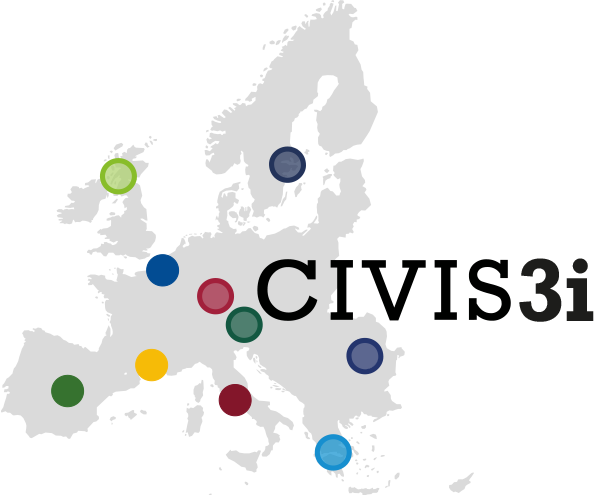
\includegraphics[width=3cm]{Logos/Civis_logo}}
  \end{tabular}    
}
\date[YGMC] % (optional, should be abbreviation of conference name)
{	
	{\vskip 1ex}
	University of Verona, Italy, January 2025
}












%---------------------------------------------------------------------------------------------------------------------------------------------------
%- D0cum3nt ----------------------------------------------------------------------------------------------------------------------------------
\begin{document}
%-------------------------------------------------------------------------------------------------------------------------------------------------
\begin{frame}  % Alternative: \maketitle outside of frame
	\titlepage
	\ifHandout
		\tikz[overlay,remember picture]
		{
	    	%	\node at ($(current page.west)+(1.5,0)$) [rotate=90] {\Huge\textcolor{gray}{\today}};
	    	\node[        
	    		draw,
	    		shape border rotate=90,
			isosceles triangle,
			isosceles triangle apex angle=90,
			fill=yellow]
	        		at ($(current page.north east)-(1,1)$) [rotate=-45] {\textcolor{red}{Handout version}};
		}
	\fi
	\end{frame}
	\addtocounter{framenumber}{-1}
\note{
	%\textbf{\underline{OUTLINE}}:
	%\tableofcontents
	\textbf{Abstract:}
	\\
%
Multisymplectic manifolds are a straightforward generalization of symplectic manifolds where closed non-degenerate k-forms are considered in place of 2-forms.
A natural theme that arises when dealing with (multi)symplectic structures is investigating the relationship between symmetries (group action preserving the fixed differential form) and reduction.

In this context, a reduction scheme can be taught as a procedure to construct a second space of reduced dimension out of a given (multi)-symplectic manifold with symmetries. The so obtained reduced space enjoys the convenient property of embodying the relevant geometric structure of the starting unreduced object.

A well-known result in symplectic geometry, known as Marsden–Weinstein–Meyer theorem, states that the relevant geometric structure of a symplectic manifold can be studied on the orbits contained in a regular level set of a so-called "momentum map".
Sniaticki and Weinstein have further extended this result to encompass singular momentum maps.

The scope of this talk is to review some relevant algebraic structures related to multisymplectic manifolds, namely the higher version of the observables algebra and moment maps, and discuss how the regular and singular reduction schemes extend to the multisymplectic framework.

This talk is based on ongoing joint work with Casey Blacker and Leonid Ryvkin.

}
%---------------------------------------------------------------------------------------------------------------------------------------------------




%-------------------------------------------------------------------------------------------------------------------------------------------------
\begin{frame}[fragile]{Keywords}
\tikzstyle{every picture}+=[remember picture]
	\begin{columns}
    	\begin{column}{.45\textwidth}
    		\onslide<4->{
			\tikz[baseline]{
		            \node[draw=orange!40,anchor=base,text width=5cm] (s1)
		            {Algebraic structure encoding informations necessary for defining coisotropic reduction in Poisson geometry.};
			}
		}
	\end{column}
    	\begin{column}{.45\textwidth}
    		\onslide<5->{
			 \tikz[baseline]{
		            \node[draw=blue!40,anchor=base, text width=5cm] (s2)
		            {Mathematical formalization of classical measurable quantities.};
			}
		}
	\end{column}
	\end{columns}

	\vfill

	\begin{center}
		\large
		 \tikz[baseline]{
		            \node[fill=orange!20,anchor=base] (t1)
		            {Constraint Algebra};
			}
		\\
		of 
		\\
		 \tikz[baseline]{
	            \node[fill=green!20,anchor=base] (t3)
	            {Multi};
		}
		\kern-3pt - \kern-3pt
		 \tikz[baseline]{
	            \node[fill=red!20,anchor=base] (t4)
	            {Symplectic};
		}		
		  \tikz[baseline]{
		            \node[fill=blue!20,anchor=base] (t2)
		            {Observables};
		        } 

	\end{center}

	\vfill

	\begin{columns}
    	\begin{column}{.45\textwidth}
    		\onslide<3->{
	 		 \tikz[baseline]{
	            \node[draw=green!40,anchor=base,text width=5cm] (s3)
	            {A certain higher version \\(involving differential forms in degree $\geq 2$)};
	         }
		}		   	
		\end{column}
    	\begin{column}{.45\textwidth}
    		\onslide<2->{
				\tikz[baseline]{
	            \node[draw=red!40,anchor=base,text width=5cm] (s4)
	            {Closed $2$-form on a smooth manifold, providing a geometric framework for classical mechanics};
	           }	
			}
		\end{column}
	\end{columns}

	\begin{tikzpicture}[overlay]
        \path[->,draw=orange!40]<4-> (s1) edge [bend right] (t1);
        \path[->,draw=blue!40]<5-> (s2) edge [bend left] (t2);
        \path[->,draw=green!40]<3-> (s3) edge [bend left] (t3);
        \path[->,draw=red!40]<2-> (s4) edge [bend left] (t4);
	\end{tikzpicture}

	\vfill
	\onslide<1->{
	\begin{block}{Based on:}
%		 \emph{ \small
%			 Blacker, M, Ryvkin;
%			\textbf{Reduction of $L_\infty$-algebra of observables on multisymplectic manifolds}; 
%			\href{https://arxiv.org/abs/2206.03137}{arXiv:2206.03137}.
%		}
%		\\
		 \emph{ \small
			 M. , Ryvkin;
			\textbf{Constraint algebras of multisyplectic observables}; 
			\href{https://www.antoniomiti.it/teaching/Obs-Constraint-2024/}{In preparation}.
		}		
	\end{block}
	}

\end{frame}
\note[itemize]{
	\item Provide a vague idea of the words that make up the title.
	\item \cite{Dippell2023}
	\item Conventions:
	\\- $M$ and $G$ are connected,
	\\- actions $\theta:G \curvearrowright M$ are always smooth
	\\- $\xi,\eta\in\g$,
	\\- for $\mu\in\Omega^*(M,\g^*)$ and $\xi\in\g$, write
			\[
				\mu_\xi := \langle\mu,\xi\rangle \;{\color{black!50}\in\Omega^*(M)}
			\]
			for the ``$\xi$th component'' of $\mu$.
}
%-------------------------------------------------------------------------------------------------------------------------------------------------



%-------------------------------------------------------------------------------------------------------------------------------------------------
\section{Symplectic Reduction}
\checkpoint	
%-------------------------------------------------------------------------------------------------------------------------------------------------

%-------------------------------------------------------------------------------------------------------------------------------------------------
\begin{frame}{Symplectic geometry (mechanics flavour)}
\begin{columns}[T]
	\begin{column}{.50\linewidth}
		\centering
		\textit{ "geometric approach" to mechanics \dots}
		%
		\begin{columns}
			\begin{column}{.60\linewidth}
				\begin{center}
					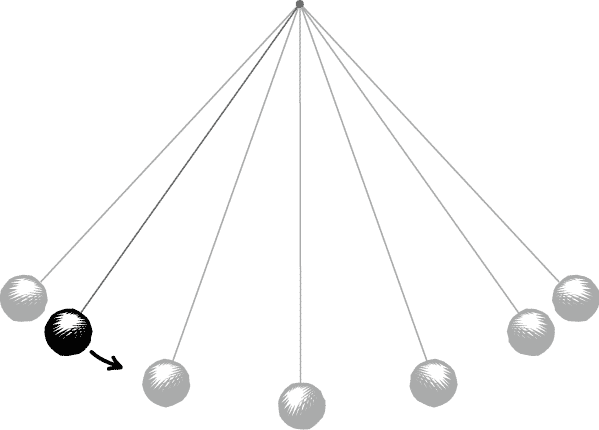
\includegraphics[width=0.6\linewidth]{Pictures/pendulum13}			
				\end{center}
			\end{column}	
			\begin{column}{.40\linewidth}
				\begin{center}
					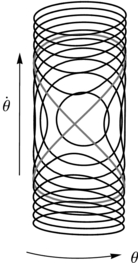
\includegraphics[width=0.45\linewidth]{Pictures/pendulum-phase-space}			
				\end{center}
			\end{column}	
		\end{columns}
		%
		\begin{defblock}[Symplectic Manifold]
			\vspace{-1em}
			\includestandalone[width=1\textwidth]{Pictures/Figure_sym}	
		\end{defblock}
		%
		\pause
		\begin{exblock}[$M = T^\ast Q$ is symplectic]
			with $\omega = d \theta $ given by
			$$ \left.\theta\right\vert_{(q,p)} (v) = p (\pi_\ast v) ~.$$
		\end{exblock}
		%
		\pause
		\vspace{1.2em}
		\centering
		\textit{ based on the notion of \\"states".}		
	\end{column}
	\onslide<1->{\vrule{}}
	\pause
	\begin{column}{.50\linewidth}
		\centering
		\textit{ "algebraic approach" to mechanics \dots}
		\vspace{.5em}	
		\begin{defblock}[Classical Observables]
			Unital, associative, commutative algebra $C^\infty(M)$.
		\end{defblock}
		%
		\vspace{.1em}
		\pause
		\begin{defblock}[Hamiltonian vector fields]
			$\vHam_f \in \mathfrak{X}(M)$ such that:
			$$\iota_{\vHam_f} \omega = -df \quad$$ %$\in B^1(M)$
			%
			\footnotetext{	$\vHam_f$ = \emph{Ham.v.f. pertaining to $f\in C^\infty(M)$}.}
		\end{defblock}
		\vspace{.1em}
		%
		\begin{defblock}[Poisson Algebra of Observables]
			$C^\infty(M)$ is a Poisson algebra with
			$$\{f,g\} = \iota_{\vHam_g} \iota_{\vHam_f} \omega = \omega(\vHam_f,\vHam_g) ~.$$
		\end{defblock}
		%
		\pause
		\vspace{.15em}
		\centering
		\textit{ based on the notion of \\"measurable quantities".}						
	\end{column}
\end{columns}
\end{frame}
\note[itemize]{
	\footnotesize

	\item We work in the framework of multisymplectic geometry which is one of the possible generalizations of the well-established field of symplectic geometry.
	
	\item To recall what symplectic geometry is let me assume a particular point of view: mechanics.
	\\
	Idea:"
	Symplectic geometry is a branch of differential geometry studying symplectic manifolds; it originated as a formalization of the mathematical apparatus of classical mechanics and geometric optics."{\href{https://ncatlab.org/nlab/show/symplectic+geometry}{nlab}}
	
	Namely, a sym. mfd. is the geometric structure encoding the phase space of conservative, ordinary, classical, mechanical systems.
	
	\item $\theta$ = \emph{tautological 1-form}.
		$\theta$ evaluated at $p\in T^*Q$ in the fibre of $q\in Q$ and contracted with $v$ coincides with the form $p$ evaluated at $q$ and contracted with the push forward of $v$.
	
	\item We identify a special class of vector fields.
		Out of them one can define a Lie bracket.
	
	\item Poisson is a Lie algebra with the extra property of compatibility with the associative product (Leibniz rule)
	
	\item take away message: geometric (based on "states") vs algebraic (based on "measurable quantities").7
}
%-------------------------------------------------------------------------------------------------------------------------------------------------

%------------------------------------------------------------------------------------------------
\begin{frame}{Reminder: momentum maps in symplectic geometry}\label{frame:symplecticmomaps}
	Consider $\theta:G\curvearrowright M$ symplectic,~~ $\underline{\cdot}:\mathfrak{g}\to \mathfrak{X}(M)$ infinitesimal action.
	\vfill

	\begin{columns}[T]
		\setlength{\belowdisplayskip}{5pt}
		\begin{column}{.50\linewidth}
			%
			\centering \it
			\onslide<2->{
				\begin{defblock}[Equivariant moment map]
					Smooth map $$\mu:M\to \mathfrak{g}^\ast$$
					such that:
					\begin{itemize}
						\item[i.] $d\langle \mu,\xi\rangle = -\iota_{\underline{\xi}}\omega$ 
						~\qquad, $\forall \xi \in \mathfrak{g}$
						\item[ii.] $\mu \circ \theta_g = Ad_g^\ast \circ \mu$
						 \qquad\small, $\forall g \in G$
					\end{itemize}
				\end{defblock}
			}
		\end{column}	
		%
		\onslide<2->{\vrule{}}
		%
		\begin{column}{.50\linewidth}
			\onslide<3->{			
				\begin{defblock}[Comoment map]
					Linear map $$\widetilde{\mu}: \mathfrak{g}\to C^\infty(M,\omega)$$
					such that:
					\begin{itemize}
						\item[i.] $d\widetilde{\mu}(\xi) = -\iota_{\underline{\xi}}\omega$ 
						\qquad~\small, $\forall \xi \in \mathfrak{g}$
						\item[ii.] $\widetilde{\mu}([\xi,\eta]) = \lbrace\widetilde{\mu}(\xi),\widetilde{\mu}(\eta)\rbrace$ \small, $\forall \xi,\eta \in \mathfrak{g}$
					\end{itemize}
				\end{defblock}
			}
		\end{column}	
	\end{columns}	
	%
	\pause
	\vspace{1em}
	%
	\begin{columns}[]
		\setlength{\belowdisplayskip}{5pt}
		\begin{column}{.40\linewidth}
			%
			\centering \it
			\onslide<5->{
				\begin{upshotblocktitle}[Duality]
					\begin{displaymath}
						\mu(x) : \mathfrak{\xi} \mapsto \widetilde{\mu}(\xi)\big\vert_x
					\end{displaymath}
					%
					\emph{
					\small
					"duality wrt. the currying operation"					
					}
				\end{upshotblocktitle}
			}
		\end{column}	
		%
		%
		\begin{column}{.60\linewidth}
			\onslide<4->{			
				\begin{upshotblocktitle}[$\widetilde{\mu}$ as a lift]
					\begin{displaymath}
						\begin{tikzcd}[ampersand replacement = \&]
						 \& C^\infty(M,\omega) \ar[d,"\vHam"]
						 \\
						 \mathfrak{g} \ar[ur,dashed,sloped,"\widetilde{\mu}"]\ar[r,"\underline{\cdot}"'] \& \mathfrak{X}(M)
						\end{tikzcd}
					\end{displaymath}
					%
					\emph{
					\small
					"it is a lift (in the Lie category) of the infinitesimal action by the assigment of hamiltonian v.fields."					
					}
				\end{upshotblocktitle}
			}
		\end{column}	
	\end{columns}		
\end{frame}
\note[itemize]{
	\item consider an action preserving the symplectic form.
	\item[-] $\langle \cdot, \cdot \rangle$ is the natural pairing of $\mathfrak{g}$ and $\mathfrak{g}^\ast$.
		\item[-] $\theta_g$ is the diffeomorphism associated to $g\in G$ via $\theta:G\curvearrowright M$
		\item[-] $Ad^\ast_g$ is the coadjoint action $G\curvearrowright \mathfrak{g}^\ast$
	\item The moment map can be reexpressed as a comomentum map.
	\item Observe that ii. on the left always implies ii. on the right. The converse is trure only if $G$ is connected.
	\item $G\curvearrowright M$ is said "Hamiltonian" (see slide \ref{frame:gisthamaction} in appendix) iff $\exists$ comoment map $\widetilde{\mu}$.
	\item \emph{moment map: Describe ${\color{orange}G\curvearrowright M}$ in terms of $\color{blue}C^\infty(M)\to\X(M)$.}
	\begin{center}
	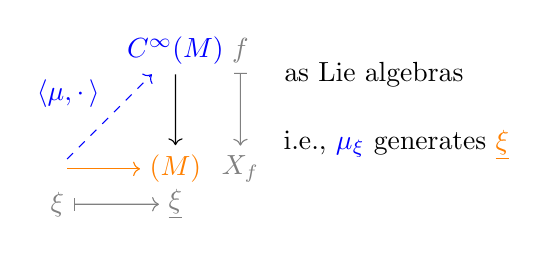
\begin{tikzpicture}[scale=1.5]
		\node[orange] (A) at (0,0) {$\g$};
		\node[gray] (A1) at (0,-.3) {$\xi$};
		\node[blue] (B) at (1,1) {$C^\infty(M)$};
		\node[gray] (B2) at (1.55,1) {$f$};
		\node[orange] (C) at (1,0) {$\X(M)$};
		\node[gray] (C1) at (1,-.3) {$\underline\xi$};
		\node[gray] (C2) at (1.55,0) {$X_f$};

		\path[->,blue,dashed] (A) edge node[above left] {$\langle\mu,\cdot\,\rangle$} (B);
		\path[->,orange] (A) edge (C);
		\path[->] (B) edge (C);
		\path[|->,gray] (A1) edge (C1);
		\path[|->,gray] (B2) edge (C2);

		\begin{scope}[xshift=3cm]
			\node at (-.32,.8) {as Lie algebras};
			\node at (-.13,.2) {i.e., {\color{blue}$\mu_\xi$} generates {\color{orange}$\underline\xi$}};
		\end{scope}
	\end{tikzpicture}
	
		\footnotesize		(\emph{moment map:} ${\color{blue}\mu:M\to\g^*}$, 
	 \emph{Hamiltonian $G$-space:} 	$(M,\omega,G,\mu)$)
	\end{center}
	\item
	 $\alpha\mapsto X_\alpha$ is a homomorphism of Leibniz algebras:
	$$\d\{\alpha,\beta\} = \d\L_{X_\alpha}\beta = \L_{X_\alpha}\iota_{X_\beta}\omega = \iota_{[X_\alpha,X_\beta]}\omega ~{\color{black!80} \implies}~
	X_{\{\alpha,\beta\}} = [X_\alpha,X_\beta]$$
}
%------------------------------------------------------------------------------------------------

\subsection{Regular reduction}
%------------------------------------------------------------------------------------------------
\begin{frame}{Regular reduction in symplectic geometry}
	\textbf{\color{UniGreen}Symplectic reduction:}~~
	\\ 
	{\it \small
	Procedure associating to any (suitably regular) pair of symplectic manifold and Hamiltonian action another symplectic manifold of smaller dimension.}
	\vfill
	\pause
	\begin{thmblock}[Marsden-Weinstein reduction \cite{MarsdenWeinstein74}]
		\vspace{-.4em}\hspace{-1em}
		\begin{tabular}{l p{14cm}}
		    Given: & $(M,\omega)$ symplectic
		    \\
		    & $G\curvearrowright M$ symplectic with equivariant momap. $\mu:M\to \mathfrak{g}^*$
		    \\[.2em]
		    Assume: & $\phi \in \mathfrak{g}^*$ regular value of $\mu$ 
		    \qquad\quad \footnotesize \textcolor{gray}{($\Rightarrow$ $\mu^{-1}(\phi)\hookrightarrow M$ smooth embedding)}
		    \\
			& $G_\phi\curvearrowright \mu^{-1}(\phi)$ free and proper
			\quad \footnotesize \textcolor{gray}{($\Rightarrow$ $\mu^{-1}(\phi)/G_\phi$ smooth manifold)}
			\\[.4em]
			Then: & $\exists!$ symplectic structure $\omega_\phi$ in $M_\phi:= \mu^{-1}(\phi)/G_\phi$ \\
			& s.t. $\pi^\ast \omega_\phi = j^\ast \omega$ 
			\qquad {\footnotesize with $j:\mu^{-1}(\phi) \hookrightarrow M$ and $\pi:\mu^{-1}(\phi)\twoheadrightarrow M_\mu$}
		\end{tabular}
		\vspace{-.4em}
	\end{thmblock}
	%
	\vfill
	\pause
	\begin{columns}
		\begin{column}{0.40\textwidth}
			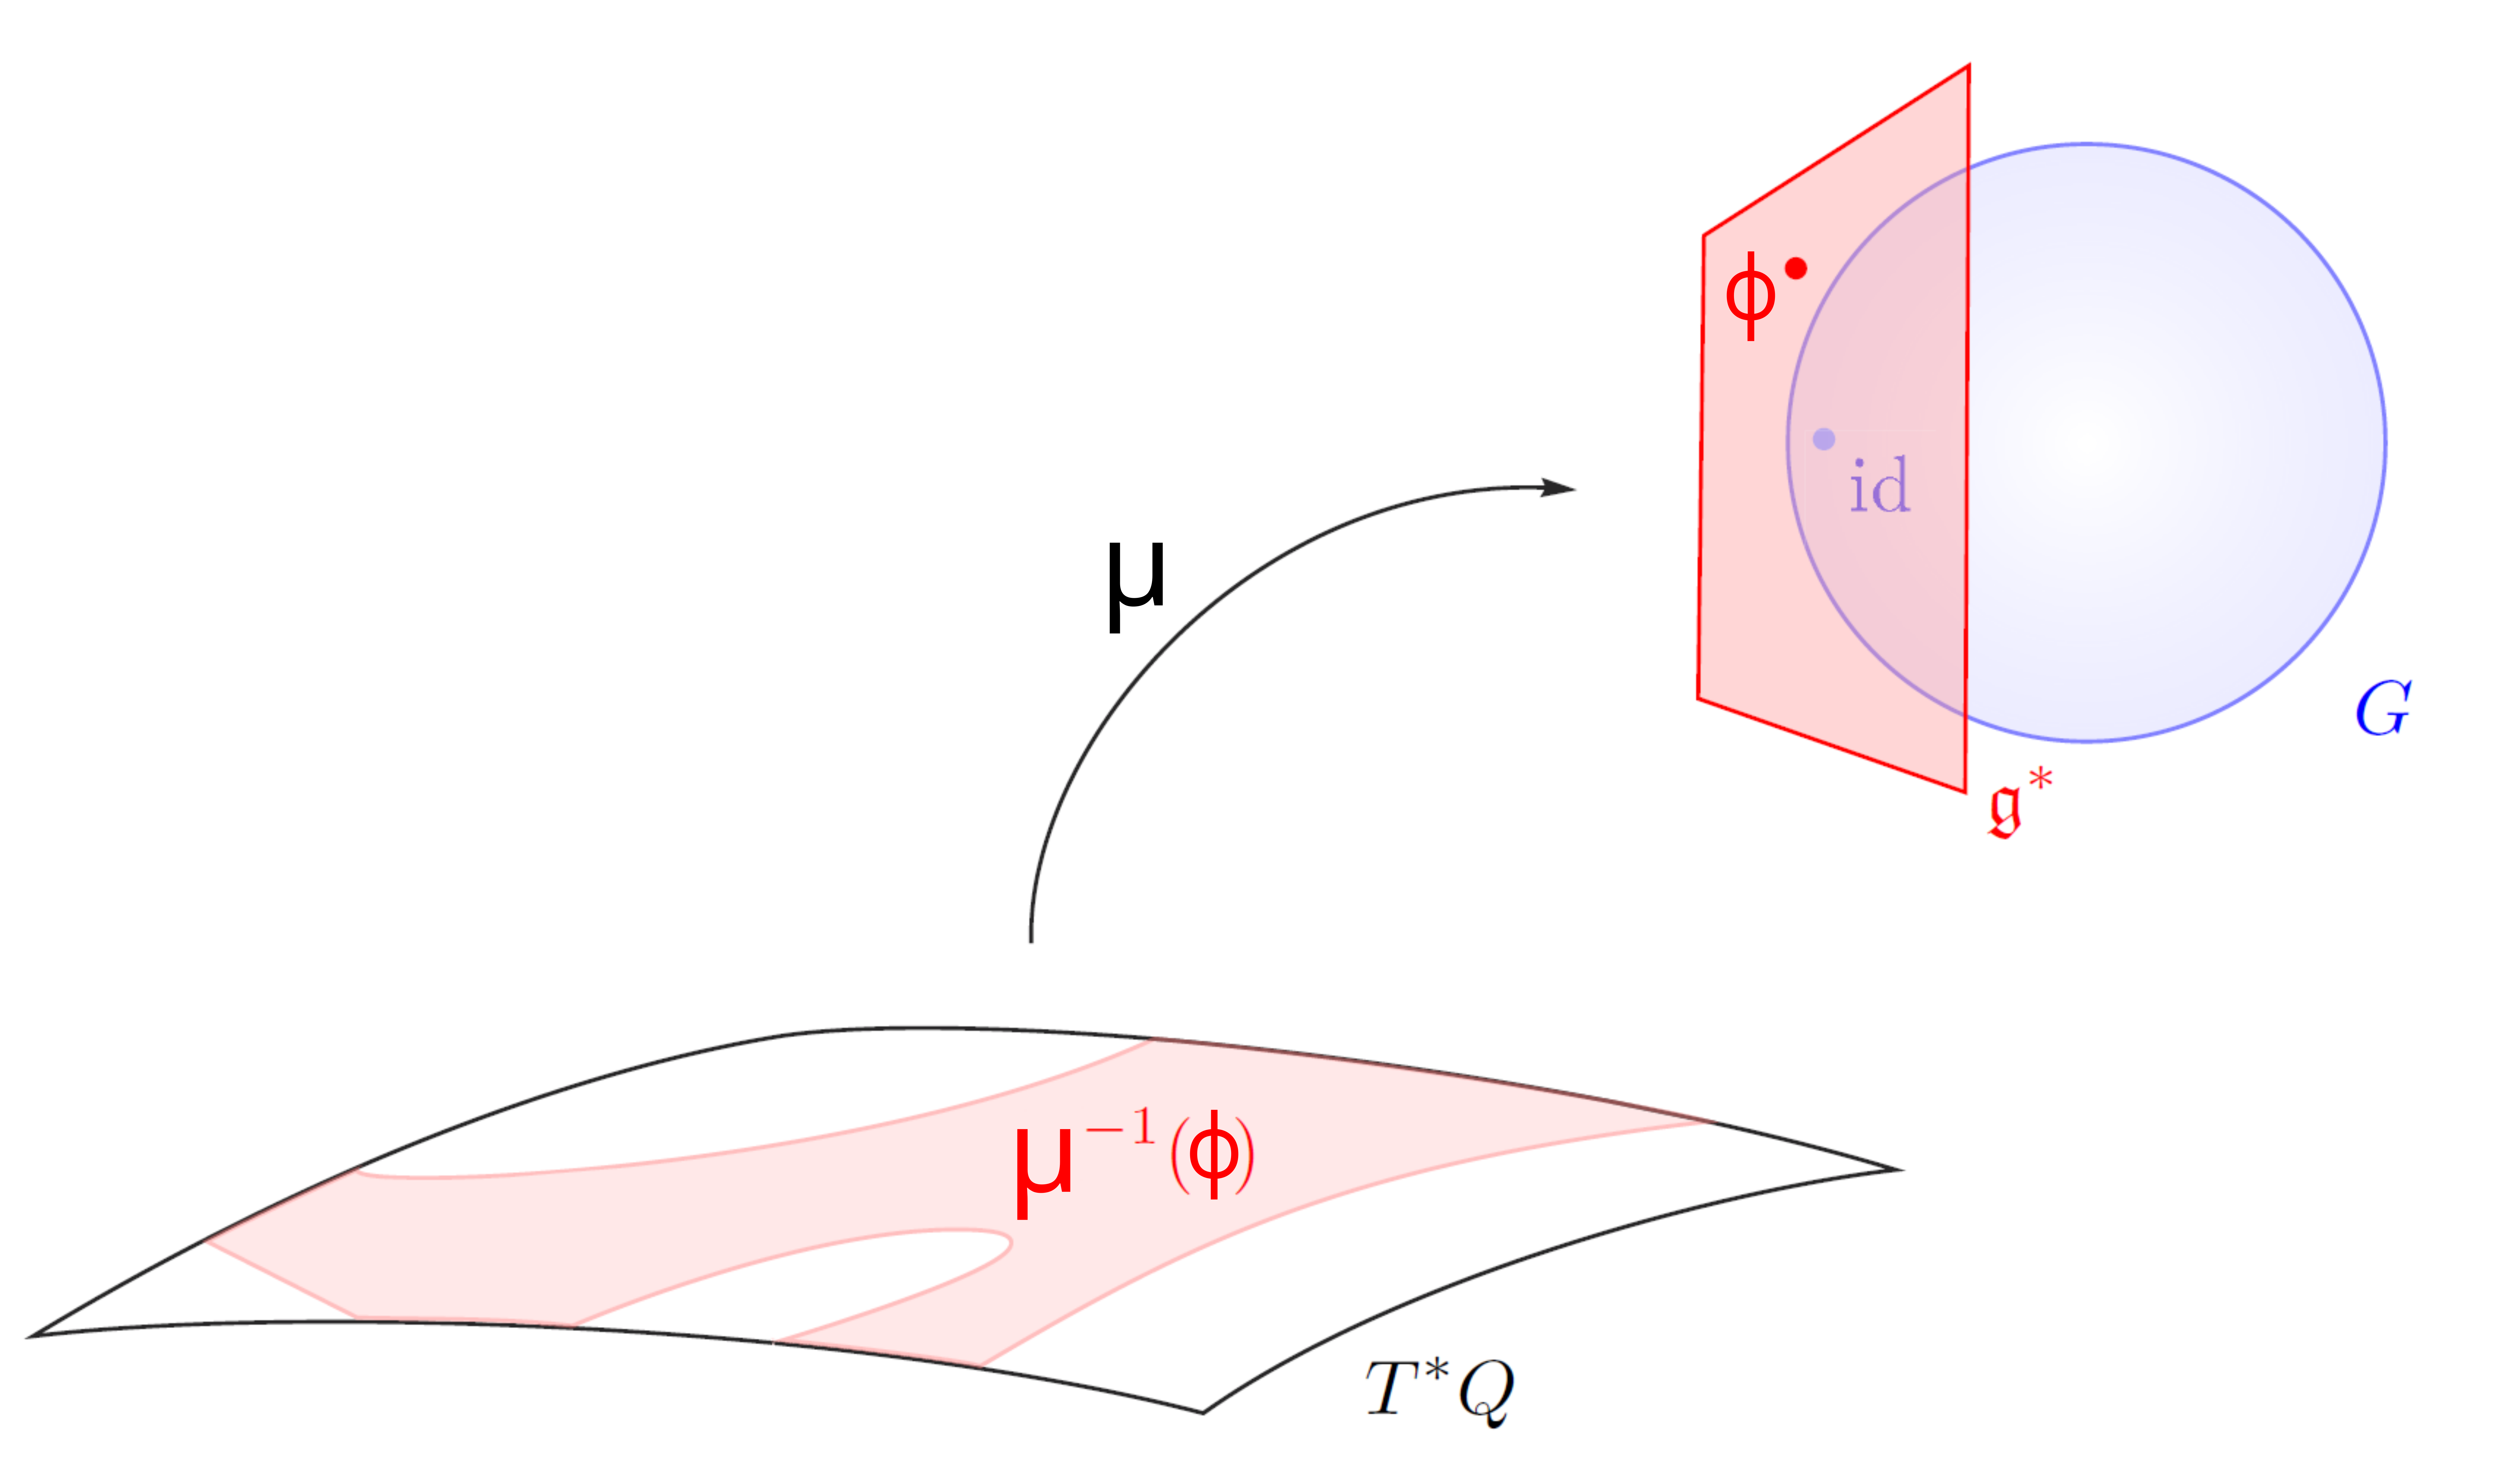
\includegraphics[width=\textwidth]{Pictures/Reduction}
		\end{column}	
		
		\begin{column}{0.6\textwidth}
				\textbf{\color{UniGreen}In mechanics:}~~
				\\
			{\it \small
				it embodies the process of restricting the dynamics of the system to the level sets of the conserved quantities pertaining to the symmetry group.		
			}
			\\[.2em]
			\color{gray}\small( e.g. restricting to studying a point-like particle in a central potential by studying it in radial coordinates)
		\end{column}	
	\end{columns}	
\end{frame}
\note[itemize]{
	\item {Symplectic Reduction} takes two inputs:
	\\ 1. Hamiltonian $G$-space $(M,\omega,{\color{orange}G},{\color{blue}\mu})$
	\\ 2. parameter ${\color{blue}\phi}\in\g^*$
	\item The \emph{reduced space} is $M_\phi:={\color{blue}\mu^{-1}(\phi)}{\color{orange}/G_\phi}$.
	\item (Marsden--Weinstein '74, Meyer '73) THM:\\
		If $\mu^{-1}(\phi)\subset M$ is smooth and $G_\phi\curvearrowright \mu^{-1}(\phi)$ is free and proper, then there is a \textbf{unique symplectic form} $\omega_\phi\in\Omega^2(M_\phi)$ such that $\pi^*\omega_\phi = i^*\omega$.


	\begin{center}
	\begin{tikzpicture}[scale=2]
		\node[blue] (A) at (0,0) {$\mu^{-1}(\phi)$};
		\node[gray] (A1) at (0,.3) {$i^*\omega$};
		\node[gray] (A2) at (-.6,0) {$\pi^*\omega_\phi$};
		\node[blue] (B) at (1,0) {$M$};
		\node[gray] (B1) at (1,.3) {$\omega$};
		\node[orange] (C) at (0,-.8) {$M_\phi$};
		\node[gray] (C2) at (-.6,-.8) {$\omega_\phi$};

		\path[right hook->,blue] (A) edge node[above] {$i$} (B);
		\path[orange,->] (A) edge node[left] {$\pi$} (C);
		\begin{scope}[xshift=-1.8cm]
			\node[blue] at (0,0) {\small restrict to $\{\mu=\phi\}$};
			\node[orange] at (.15,-.4) {\small quotient by $G_\phi$};
		\end{scope}
	\end{tikzpicture}
	\end{center}
	\item Heuristic Approach to Reduction:
	\\1. describe $G\curvearrowright M$ in terms of $\omega$ 	\hspace{1cm}
	({\color{green}moment map $\mu$})
	\\2. identify a distinguished reduced space \hspace{1cm}
	({\color{green}reduction at $\mu=0$})
	\\3. use the ambiguity in 1.\ to obtain a family of reduced spaces \hspace{1cm}
	({\color{green}reduction at $\mu-\phi=0$, i.e.\ reduction at $\mu=\phi$}
	\\
	{\tiny Note: If $G_\phi\neq G$, then $\mu-\phi:M\to\g^*$ is not a moment map for either $G\curvearrowright M$ or $G_\phi\curvearrowright M$.}
	
}
%------------------------------------------------------------------------------------------------

%-------------------------------------------------------------------------------------------------------------------------------------------------
\subsection{Singular reduction}
\begin{frame}{Symplectic singular reduction schemes}
	\begin{block}{The gist of singular reduction}
 		\begin{itemize}
 			\item[-] when $\mu$ is singular (i.e. $\mu^{-1}(0)$ is not a mfd.), the (geometrically) reduced space may not exist.
 			\item[-] a \emph{singular reduction scheme} is a procedure to construct a "reduced" algebra of observable out of the given data
 			\item[-] such that it corresponds to the algebra of observable of the reduced manifold in the regular case.
 		\end{itemize}
	\end{block}
 	%
 	\pause
 	%
	\begin{thmblock}[Sniatycki-Weinstein reduction \cite{SniatyckiWeinstein83}]
		\vspace{-.4em}\hspace{-1em}
		\begin{tabular}{l p{14cm}}
		    Given: & $(M,\omega)$ symplectic
		    \\
		    & $G\curvearrowright M$ symplectic with equivariant momap. $\mu:M\to \mathfrak{g}^*$
			\\[.4em]
			Then: & 
			$\displaystyle \left[\sfrac{C^\infty(M)}{I_\mu}\right]^G$
			admits a Poisson algebra structure 
			\blfootnote{$I_\mu$ = associative ideal generated by $\widetilde{\mu}(\g)$}			
			\\
			& it agrees with the M--W reduction in the regular case.		
		\end{tabular}
		\vspace{-.4em}
	\end{thmblock}
 

\end{frame}
\note[itemize]{
 \item Let $(M,\omega,G,\mu)$ be a symplectic Hamiltonian $G$-space.
 \item The \emph{momentum ideal} is the associative ideal $I_\mu\subset C^\infty(M)$ generated by the momenta $\mu_{\xi}$ for any $\xi\in \mathfrak{g}$.
		Namely
		\[
			I_\mu 
			= 
			\Big\langle \mu_\xi \Big\rangle_{\xi \in \mathfrak{g}}^{\text{\tiny asso.}} 
			=
			\left\{
				\left.
					\sum_{i=1}^n f_i ~ \mu_{\xi_i}
				\right|~
					f_i \in C^\infty(M),~ \xi_i\in \mathfrak{g},~  1 \leq i \leq n
			\right\}
		\]

 \item The \emph{\'Sniatycki--Weinstein reduction} is the Poisson algebra
		\[
			\left(C^\infty(M)/I_\mu\right)^G.
		\]


}
%-------------------------------------------------------------------------------------------------------------------------------------------------



%-------------------------------------------------------------------------------------------------------------------------------------------------
\section{Multisymplectic Geometry}
\checkpoint	
%-------------------------------------------------------------------------------------------------------------------------------------------------

%-------------------------------------------------------------------------------------------------------------------------------------------------
\begin{frame}{From symplectic to {multi}symplectic} 
	%
	\begin{center}
		$-$ \emph{multisymplectic means \textbf{going higher} in the degree of $\omega$} $-$
	\end{center}
	\pause
	\begin{defblock}[$n$-plectic manifold ~\emph{(Cantrijn, Ibort, De Le\'on)} \cite{Cantrun2017}]
		\includestandalone[width=0.95\textwidth]{Pictures/Figure_multisym}	
	\end{defblock}
	%
	\pause
		\begin{table}
			\begin{tabular}{c c c}
				symplectic forms \small($n=1$) & $\leftrightsquigarrow$ & volume forms \small($n= \text{dim}(M)-1$)
			\end{tabular}
		\end{table}

	\vfill
	\pause
	\begin{block}{Historical motivation}
		Mechanics: geometrical foundations of \textit{(first-order)} field theories.
	\end{block}
	%
	\begin{table}
		\ifHandout
		%
		\else
		\only<4>{
		\begin{tabular}{|p{0.2\textwidth}|p{0.3\textwidth}|p{0.35\textwidth}|} 
            \hline
            \parbox[][20pt][c]{0.2\textwidth}{mechanics} & \multicolumn{2}{c|}{geometry} \\
            \hline
            \parbox[][20pt][c]{0.2\textwidth}{phase space} & symplectic manifold &  \\[.25em]
            \parbox[][20pt][c]{0.2\textwidth}{classical \\ observables} & Poisson algebra &  \\[.25em]
            \parbox[][20pt][c]{0.2\textwidth}{symmetries} &  group actions admitting comoment map &  
            \\
            \hline
  \multicolumn{1}{c}{}
            &  \multicolumn{1}{@{}c@{}}{$\underbrace{\hspace*{.3\textwidth}}_{\text{point-like particles systems}}$} 
            &  \multicolumn{1}{@{}c@{}}{}              \\
		\end{tabular}
		}
		\fi
		\onslide<5->{
		\begin{tabular}{|p{0.2\textwidth}|p{0.3\textwidth}|p{0.35\textwidth}|} 
            \hline
            \parbox[][20pt][c]{0.2\textwidth}{mechanics} & \multicolumn{2}{c|}{geometry} \\
            \hline
            \parbox[][20pt][c]{0.2\textwidth}{phase space} & symplectic manifold & multisymplectic manifold \\[.25em]
            \parbox[][20pt][c]{0.2\textwidth}{classical \\ observables} & Poisson algebra & $L_\infty$-algebra \\[.25em]
            \parbox[][20pt][c]{0.2\textwidth}{symmetries} &  group actions admitting comoment map & group actions admitting (homotopy) comomentum map
            \\
            \hline
  			\multicolumn{1}{c}{}
            &  \multicolumn{1}{@{}c@{}}{$\underbrace{\hspace*{.3\textwidth}}_{\text{point-like particles systems}}$} 
            &
            \multicolumn{1}{@{}c@{}}{$\underbrace{\hspace*{.3\textwidth}}_{\text{field-theoretic systems}}$} 
               \\
		\end{tabular}
		}
	\end{table}	




\end{frame}
\note[itemize]{
	\item Historically, the interest in multisymplectic manifolds, has been motivated by the need for understanding the geometrical foundations of first-order classical field theories.
	The key point is that, just as one can associate a symplectic manifold to an ordinary classical mechanical system (e.g. a single
point-like particle constrained to some manifold), it is possible to associate a multisymplectic
manifold to any classical field system (e.g. a continuous medium like a filament or a fluid). See frame Extra-\ref{Frame:Ms-Field-Mechanics} 
	
	\item General ideas basic parallelisms with caveats
	\item caveat: points in multiphase spaces are not states
	\item the table hides the duality between geometric and algebraic approaches to the problem.
	\item	Mechanics: geometrical foundations of \textit{(first-order)} field theories.
		\begin{itemize}
		 \item[-] Kijowski, W. Tulczyjew \cite{Kijowski1979}; %(1979)
		 \item[-] Cariñena, Crampin, Ibort \cite{Carinena1991b};% (1991)
		 \item[-] Gotay, Isenberg, Marsden, Montgomery \cite{Gimmsy1};%(1998)
		 \\ $\cdots$
		\end{itemize}
}
%-------------------------------------------------------------------------------------------------------------------------------------------------

%-------------------------------------------------------------------------------------------------------------------------------------------------
\begin{frame}{Observables in $n$-plectic geometry}
	%
	\begin{defblock}[Hamiltonian $(n-1)$-forms]
		\begin{displaymath}
			\Omega^{n-1}_{ham}(M,\omega) 	:=
			\biggr\{ \sigma \in  \Omega^{n-1}(M) \; \biggr\vert \; 
				\exists \vHam_\sigma \in \mathfrak{X}(M) ~:~ 
				\tikz[baseline,remember picture]{\node[rounded corners,
                        fill=orange!5,draw=orange!30,anchor=base]            
            			(target) {$d \sigma = -\iota_{\vHam_\sigma} \omega$ };
            	}				
				~\biggr\} 
			\end{displaymath}
	\end{defblock}

	\pause
		\tikz[overlay,remember picture]
		{
			\node[rounded corners,
                 fill=orange!5,draw=orange!30,anchor=base]
            	 (base) at ($(current page.north east)-(2,1)$) [rotate=-0,text width=3.5cm,align=center] {\footnotesize{\textcolor{red}{Hamilton-DeDonder-Weyl \\equation}}};
		}	
	\begin{tikzpicture}[overlay,remember picture]
    	\path[->] (base.south) edge[bend right,red](target.north);
    \end{tikzpicture}
	%
	\vfill
	\begin{columns}[T]
		\pause
		\setlength{\belowdisplayskip}{5pt}
		\begin{column}{.50\linewidth}
			%
			\vspace{-1em}
			\begin{thmblock}[Observables $L_\infty$-algebra]
				$\Omega^{n-1}_{ham}(M,\omega)$ endowed with
				\vspace{-.5em}
				\begin{displaymath}
					\lbrace \sigma_1, \sigma_2 \rbrace =			
					~ - \iota_{\vHam_1}\iota_{\vHam_2} \omega 
				\end{displaymath}			
				can be "completed" to a \\ $L_\infty-algebra$.
			\end{thmblock}
			%	
		\end{column}	
		%
		\pause
		\begin{column}{.50\linewidth}
		%
			\begin{itemize}
				\item[\cmark] Skew-symmetric;
				\item[\xmark] multiplication of observables;
				\item[\xmark] Jacobi equation;
				%\\ \hspace*{4.25em} full-fledged Jacobi equation;
				\item[\smark] Jacobi equation \emph{up to homotopies}.
			\end{itemize}			
			%
				\[
					\small
					\{\alpha,\{\beta,\gamma\}\} + \text{\it cyc. perm.}
					= {\color{orange}\d \iota_{X_\alpha} \iota_{X_\beta} \iota_{X_\gamma}\omega}
				\]
		\end{column}	
	\end{columns}
	%
	\vfill
	\pause
	Interesting alternatives:
	\begin{itemize}
		\item  descend to $\Omega^{k-1}_{ham}(M) / {\color{orange}\d\hspace{1pt}\Omega^{k-2}(M)}$, hence getting a Lie algebra;
		\item Incorporate the {\color{orange}discrepancy} as part of the data of the space of observables $ 
				L_\infty(M,\omega) = \Omega_{ham}^{k-1}(M)\oplus{\color{orange}\Omega^{\leq k-2}(M)}$
			%a \textbf{homotopy Lie algebra} or \textbf{$L_\infty$-algebra}.
	\end{itemize}
	
	
\end{frame}
\note[itemize]{
	\item
}
%-------------------------------------------------------------------------------------------------------------------------------------------------




%---------------------------------------------------------------------------------------------------------------------------------------------------
\subsection{$L_\infty$-algebra of Observables}
\begin{frame}[fragile,t]{$L_\infty$-algebra of Observables (higher observables) }
	Let be $(M,\omega)$ a $n$-plectic manifold.
	\begin{defblock}[$L_\infty$-algebra of observables ~\emph{(Rogers)} ~\cite{Rogers2010}]
		
		\hspace{.25em} $L\infty(M,\omega)$ is given by:
		
		\begin{itemize}
			\item[•] a cochain-complex $(L,\{\cdot\}_1)$ 
		\end{itemize}
		\begin{center}
		\ifHandout
			\includestandalone{Pictures/Figure_Observables}	
		\else
			\includestandalone{Pictures/Frame_Observables}
		\fi				
		\end{center}
		\onslide<2->{
			\begin{itemize}
				\item[•] with $n$ (skew-symmetric) multibrackets $(2 \leq k \leq n+1)$
			\end{itemize}
			\begin{center}
				\includestandalone{Pictures/Equation_Multibracket}	
			\end{center}
		}
		%
	\end{defblock}
  \end{frame}
 \note[itemize]{
	\item if symplectic manifolds are the symmetric take on mechanics, Poisson algebras are the algebraic counterpart.
 	\item A Lie algebra is associated to an ordinary symplectic manifold (its Poisson algebra).
	%(Underlying this is a Lie algebra, whose Lie bracket is the Poisson bracket.)
	Similarly, one associates an Lie-$n$ algebra to any $n$-plectic manifold.
 	% https://ncatlab.org/nlab/show/n-plectic+geometry 	 
 	 %https://ncatlab.org/nlab/show/Poisson+bracket+Lie+n-algebra
	 \item Basically, the higher observables algebra is a chunk of the de Rham complex of $M$ with inverted grading( convention employed here) and an extra structure called "multibrackets".
 	\item ( In the 1-plectic case it reduces to the corresponding Poisson algebra of classical observables)
 	\item Rogers associated to any n-plectic mfd a $L\-\infty$ algebra, Zambon generalized it to the pre-n-plectic case.
 	\item Recognize in the definition of $\{\cdot,\ldots,\cdot\}_k$ the contraction with hamiltonian fields $v_\sigma$ w.r.t. $\sigma$.
  	\item Note $	\iota_{v_{\sigma_1}}\cdots\iota_{v_{\sigma_k}} = (-)^{(k-1)+(k-2)+\dots+1}\iota_{v_{\sigma_k}}\cdots\iota_{v_{\sigma_1}} = (-)^{\frac{k(k-1)}{2}}\iota_{v_{\sigma_k}}\cdots\iota_{v_{\sigma_1}}$ 
 	The definition usually find in literature of Rogers multibrackets involves the coefficient $ (-)^{\frac{k(k-1)}{2}} = -\varsigma(k-1) = (-)^{k+1} \varsigma(k)$.
  \item higher observables is Special instance of a more general object  called $L\-\infty$ Algebra...
 }
%------------------------------------------------------------------------------------------------

%------------------------------------------------------------------------------------------------
\end{document}

%-------------------------------------------------------------------------------------------------------------------------------------------------
\section{Multisymplectic observables reduction}
\checkpoint	
%-------------------------------------------------------------------------------------------------------------------------------------------------
%-------------------------------------------------------------------------------------------------------------------------------------------------
\begin{frame}{Singular Reduction: Roadmap}
	%
	\begin{block}{Data:}
			\begin{itemize}
				\item A \emph{constraint set} $N$ (possibly singular),
				\item An infinitesimal action preserving $N$.
			\end{itemize}
	\end{block}
	%
	\vfill
	\pause
	%
	\begin{block}{Goal:}
		\begin{itemize}
			\item Obtain a "reduced" observables algebra out of the data.
		\end{itemize}
	\end{block}
	%
	\vfill
	\pause
	%
	\begin{block}{Strategy:}
		\begin{enumerate}
			\item Define smooth fields/forms \emph{tangent to $N$},
			\item define smooth fields/forms \emph{vanishing along $N$},
			\item define \emph{reducible fields} requiring the preservation of the vanishing objects,
			\item define \emph{reducible forms} requiring their conservation w.r.t. the infinitesimal action,
			\item define \emph{reducible and vanishing observables},
			\item \textbf{quotient}
		\end{enumerate}
	\end{block}






\end{frame}
\note[itemize]{
	\item
}

%-------------------------------------------------------------------------------------------------------------------------------------------------


%-------------------------------------------------------------------------------------------------------------------------------------------------
\begin{frame}[shrink]{Smooth objects on a singular set}
	Consider $N$ closed subset of $M$.
	\vfill
	\pause
	\begin{defblock}
	 $I_N$ = ideal of smooth functions vanishing over $N$.
	\end{defblock}
	\vfill
	\pause

	\begin{columns}[T]
		\setlength{\belowdisplayskip}{5pt}
		\begin{column}{.65\linewidth}
			%
			\centering \it
				\begin{defblock}[v.f tangent to $N$]
					\begin{displaymath}
						\X_N(M):=
						\left\lbrace
							v \in \X(M)
						~\Big\vert~
							\L_v(I_N) \subseteq I_N
						\right\rbrace
					\end{displaymath}
				\end{defblock}
				\begin{defblock}[v.f vanishing on $N$]
					\begin{displaymath}
						I_\X(N):=
						\left\lbrace
							v \in \X(M)
						~\Big\vert~
							\L_v(C^\infty(M)) \subseteq I_N
						\right\rbrace
					\end{displaymath}				
				\end{defblock}				
		\end{column}	
		%
		%
		\begin{column}{.35\linewidth}
			\centering 
			\includestandalone[width=0.8\textwidth]{Pictures/Figure_VfTangentN}			
		\end{column}	
	\end{columns}			
	%	
	\pause

				%

				%	
		\begin{tcolorbox}[
		enhanced,frame hidden,borderline={0.5pt}{0pt}{blue},
		arc=5pt,colback=white,
		colbacktitle=white,]
			\color{blue}{\textbf{Lem}:} If $N$ is smoothly embedded,  $\X(N)\cong {X_N(M)}/{I_\X}$.
		\end{tcolorbox}

		\pause

		\begin{defblock}[Differential form vanishing on $N$]
			\begin{displaymath}
				I_{\Omega(N)}:=
				\left\lbrace
					\alpha\in\Omega^k(M
				~\left\vert~
					\begin{array}{l r}
						k\geq 0,~		\\		
						\alpha(u_1,\ldots,u_k) \in I_N & \forall u_i \in\X_N(M)
					\end{array}
				\right\rbrace\right.
			\end{displaymath}
		\end{defblock}

\end{frame}
\note[itemize]{
 \item $N$ is not a submanifold in general. An example is $N=\mu^{-1}(0)$ for a certain smooth map $N$.
 \item observe that if $N$ is a smooth embedded submanifold, one has that $\X(N)\cong \frac{X_N(M)}{I_\X}$  

}
%-------------------------------------------------------------------------------------------------------------------------------------------------



%-------------------------------------------------------------------------------------------------------------------------------------------------
\subsection{Multisymplectic singular reduction}
\begin{frame}{Reducible smooth objects \quad \small (w.r.t. $N$ and $\g\action M$)}
	Consider $\g \action M$ by vector fields tangent to $N$ % \hfill( fond. distribution $\underline{\g}\subseteq \X_N(M)$)
	\\
	\vfill
	Denote by :  
	\hspace{1em} $\underline{\g}\subseteq \X_N(M)$ the fundamental distribution,
	\\
	\hspace{6.5em}  $\X_g$ the $C^\infty$-module generated by $\underline{\g}$.
	\\
	\vfill
	\begin{defblock}[Reducible v.fields ]
			\begin{displaymath}
				\X(M)_{[N]} :=
				\left\lbrace
					v \in \X(M)
				~\left\vert~
					\begin{array}{l}
						\L_v (I_N) \subseteq I_N	\\		
						\L_v (\X_g) \subseteq \X_g + I_\X
					\end{array}
				\right\rbrace\right.
			\end{displaymath}
%			\blfootnote{
%			 $\X_g$ = $C^\infty(M)$-module generated by the fundamental distribution.
%			}	

	\end{defblock}	
	%
	\pause
	%
	\begin{defblock}[Reducible forms ]
		\begin{displaymath}
			\Omega(M)_{[N]} :=
			\left\lbrace
				\alpha \in \Omega(M)
			~\left\vert~
				\begin{array}{l r}
					\L_\underline{\xi} \,\alpha \in I_{\Omega(N)}	\\		
					\iota_\underline{\xi} \,\alpha \in I_{\Omega(N)}	& \forall \xi \in \g				\end{array}
			\right\rbrace\right.
		\end{displaymath}	
	\end{defblock}	
	%
	\pause
	\vfill
	%
	Let $(M,\omega)$ be a $k$-plectic manifold
	\begin{defblock}[Reducible Hamiltonian forms]
		\begin{displaymath}
			(\Omega(M)_{ham}^{n-1})_{[N]} :=
			\left\lbrace
				\alpha \in \Omega(M)_{ham}^{n-1}
			~\left\vert~
				\begin{array}{l r}
					\alpha \text{ is a reducible form} \\
					\vHam_\alpha \text{ is a reducible v.field}
				\end{array}
			\right\rbrace\right.
		\end{displaymath}	
	\end{defblock}		

	
\end{frame}
\note[itemize]{
 \item $\g\action M$ by vector field tangent to $N$ means that $\underline{\xi}\in\X_n(M) \forall \xi \in \g$
 \item Spelling out the definition: reducible vector fields are 
 \\i) v.f. tangent to N 
 \\ii) such that their commutator with any $\underline{\xi}$ lies in $\X_\g$ along $N$.
 \item more algebraically, they stabilize both $I_N$ and $\X_g + I_\X$.
 \item observe that $\L_v I_\X \subseteq I_\X$ since , $\forall u \in I_\X$ $\forall f \in C^\infty(M)$ one has\\
 $(\L_v u) f = \L_{[v,u]} f = \L_v\L_u f - \L_u\L_v f \in I_N$
 \item
}
%-------------------------------------------------------------------------------------------------------------------------------------------------

%-------------------------------------------------------------------------------------------------------------------------------------------------
\begin{frame}\frametitle{Hierarchy of auxiliary constructions}
	\begin{minipage}{\textwidth}
	\centering
	\scalebox{.65}{
	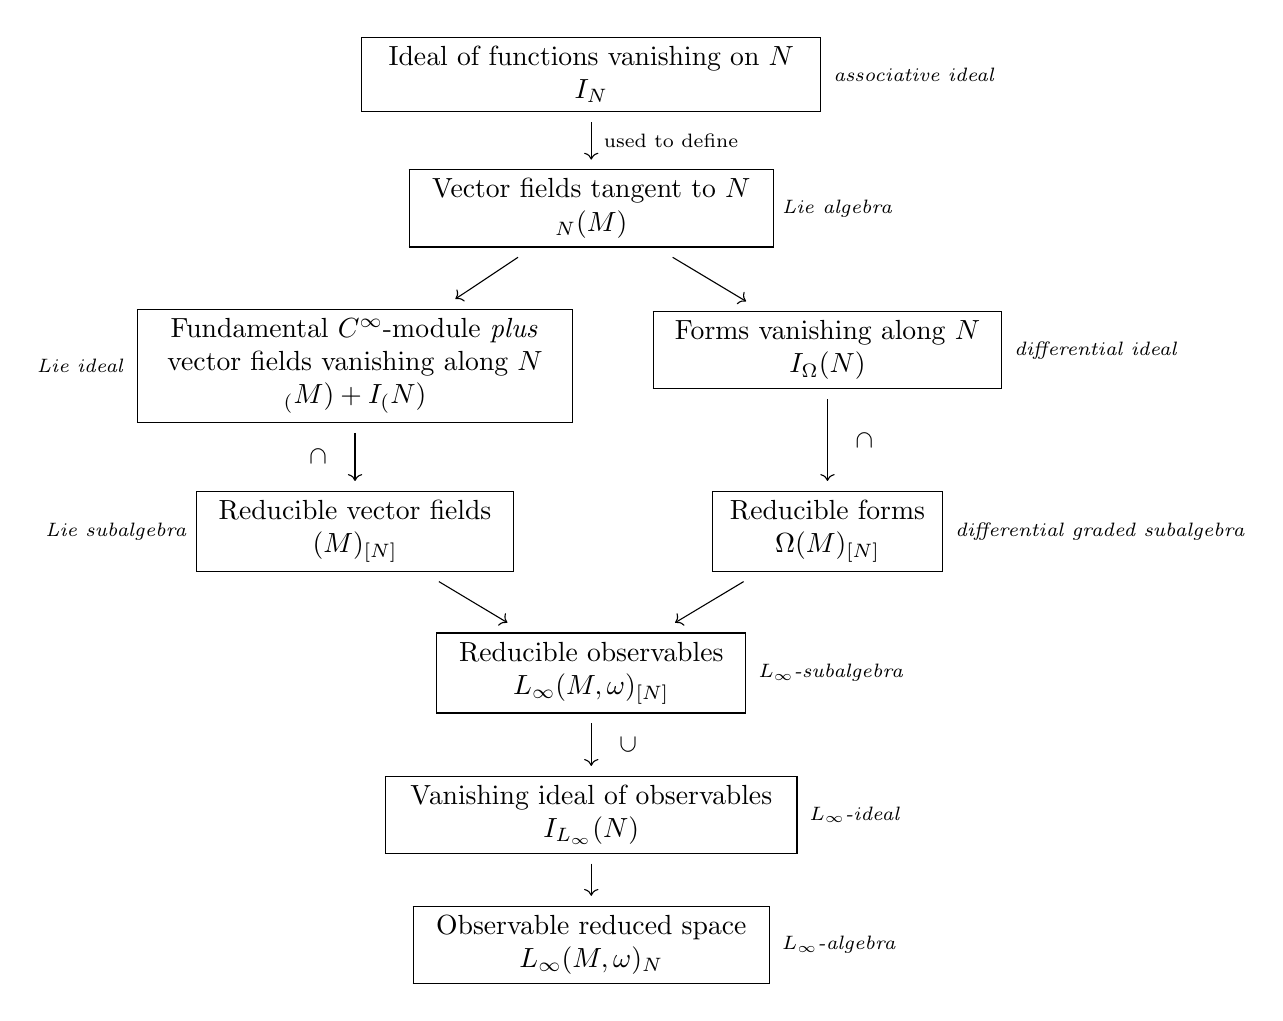
\begin{tikzpicture}
		\node (A) at (0,10.0) {\fbox{\parbox{5.6cm}{\centering Ideal of functions vanishing on $N$ \\ $I_N$}}};
		\node (B) at (0,8.3) {\fbox{\parbox{4.4cm}{\centering Vector fields tangent to $N$ \\ $\X_N(M)$}}};
		\node (C) at (3,6.5) {\fbox{\parbox{4.2cm}{\centering Forms vanishing along $N$ \\ $I_\Omega(N)$}}};
		\node (D) at (3,4.2) {\fbox{\parbox{2.7cm}{\centering Reducible forms \\ $\Omega(M)_{[N]}$}}};
		\node (E) at (-3,6.3) {\fbox{\parbox{5.3cm}{\centering Fundamental $C^\infty$-module \emph{plus} \\ vector fields vanishing along $N$ \\ $\X_\g(M)+I_\X(N)$}}};
		\node (E') at (-3,4.2) {\fbox{\parbox{3.8cm}{\centering Reducible vector fields \\ $\X(M)_{[N]}$}}};
		\node (F) at (0,2.4) {\fbox{\parbox{3.7cm}{\centering Reducible observables \\ $L_\infty(M,\omega)_{[N]}$}}};
		\node (G) at (0,0.6) {\fbox{\parbox{5.0cm}{\centering Vanishing ideal of observables \\ $I_{L_\infty}(N)$}}};
		\node (H) at (0,-1.05) {\fbox{\parbox{4.3cm}{\centering Observable reduced space \\ $L_\infty(M,\omega)_N$}}};

		\draw[->] (A)-- node[right=1pt]{{\scriptsize used to define}} (B);
		\draw[->] (B)-- (C);
		\draw[->] (C)-- node[right=.25cm]{\rotatebox{-90}{\small $\subset$}} (D);
		\draw[->] (B)-- (E);
		\draw[->] (D)-- (F);
		\draw[->] (E)-- node[left=.25cm]{\rotatebox{-90}{\small $\subset$}} (E');
		\draw[->] (E')-- (F);
		\draw[->] (F)-- node[right=.25cm]{\rotatebox{90}{\small $\subset$}} (G);
		\draw[->] (G)-- (H);

		\node[right=2.95cm] at (A) {\scriptsize\emph{associative ideal}};
		\node[right=2.30cm] at (B) {\scriptsize\emph{Lie algebra}};
		\node[right=2.25cm] at (C) {\scriptsize\emph{differential ideal}};
		\node[right=1.5cm] at (D) {\scriptsize\emph{differential graded subalgebra}};
		\node[left=2cm] at (E') {\scriptsize\emph{Lie subalgebra}};
		\node[left=2.8cm] at (E) {\scriptsize\emph{Lie ideal}};
		\node[right=2cm] at (F) {\scriptsize\emph{$L_\infty$-subalgebra}};
		\node[right=2.65cm] at (G) {\scriptsize\emph{$L_\infty$-ideal}};
		\node[right=2.3cm] at (H) {\scriptsize\emph{$L_\infty$-algebra}};
	\end{tikzpicture}
	}
	\end{minipage}
\end{frame}
\note[itemize]{
 \item
}

%-------------------------------------------------------------------------------------------------------------------------------------------------

%-------------------------------------------------------------------------------------------------------------------------------------------------
\begin{frame}{Multisymplectic observable reduction}
	\begin{defpropblock}[Reducible $L_\infty$-observables]
		Is the {\color{blue!70!black}$L_\infty$-subalgebra} of $L_\infty(M,\omega)$ given by
		\begin{displaymath}
			L_\infty(M,\omega)_{[N]}^k :=
			\begin{cases}
				\Omega^{n-1-k}(M)_{[N]} 
				\qquad\text{\color{gray}\small (reducible forms) }
				& \text{if } n-1\leq k < 0 \\
				(\Omega(M)_{ham}^{n-1})_{[N]} 
				\quad
				\text{\color{gray}\small (reducible hamiltonians) }
				& \text{if } k = 0 \\
				0 & \text{if } k > 0
			\end{cases}
		\end{displaymath}
	\end{defpropblock}
	%
	\pause
	%
	\begin{defpropblock}[Vanishing $L_\infty$-observables]
		Is the {\color{blue!70!black}$L_\infty$-ideal} of $L_\infty(M,\omega)_{[N]}$ given by
		\begin{displaymath}
			I_{L_\infty(M,\omega)} :=
			\left\lbrace
				\alpha \in L_\infty(M,\omega)_{[N]}
			~\left\vert~
				\begin{array}{l l}
					\alpha(v_1,\dots,v_k) \in I_N  \quad \forall v_i \in \X_N &
					\text{if}~ \alpha \in \Omega^k \\
					\vHam_\alpha \in \X_\g + I_\X &
					\text{if}~ \alpha \in \Omega^{n-1}
				\end{array}
			\right\rbrace\right.
		\end{displaymath}
	\end{defpropblock}
	%
	\pause
	%
	\begin{thmblock}[Blacker - M. - Ryvkin]%[Reduced $L_\infty$-algebra of observables]
		The reduction of $L_\infty(M,\omega)$  with respect to $\g\curvearrowright (N\subset M)$ is the %$L_\infty$-algebra
		quotient
		\begin{displaymath}
					L_\infty(M,\omega)_N = \frac{L_\infty(M,\omega)_{[N]}}{I_{\L_\infty}(N)}~.		
		\end{displaymath}
	\end{thmblock}

\end{frame}
\note[itemize]{
 \item The graded vector space underlying the reduced $L_\infty$-algebra $\Ham_\infty(M,\omega)_N$ is explicitly given by
\begin{displaymath}
	\Ham_\infty(M,\omega)_N =
	\frac{
		\left\lbrace
			(\alpha,v) \in \Omega(M){[n{-}1]}\oplus\X(M)
		~\left\vert~
			\begin{array}{l l}
				\iota_v \omega = -\d \alpha^{(0)} &
				\\
				\iota_\xi \alpha \in I_{\Omega}(N) &
				\\
				\L_\xi\alpha \in I_{\Omega}(N)
				&
				\\
				\L_\xi v \in \fgmodule +\vanvf
				&~\forall \xi \in \g 
				\\
				v \in \X_N(M)
				&
			\end{array}
		\right.
		\right\rbrace
	}{
		\left\lbrace
			(\alpha,v) \in \Omega(M){[n{-}1]}\oplus\X(M)
		~\left\vert~
			\begin{array}{l}
				\alpha \in I_{\Omega}(N)
				\\
				v \in \fgmodule +\vanvf
			\end{array}
		\right.
		\right\rbrace
	}~.
\end{displaymath}
}
%-------------------------------------------------------------------------------------------------------------------------------------------------

%-------------------------------------------------------------------------------------------------------------------------------------------------
\begin{frame}{Singular reduction (Conclusions)}
		  \centering 
	\emph{Reduction of states vs.\ reduction of observables}
	\vfill
	\begin{minipage}{.7\textwidth}
	\hspace{-.4cm}
	\begin{tikzpicture}
		\draw (-4,-2.5) rectangle (4,2.5);
		\draw (-4,0) -- (4,0);
		\draw (0,-2.5) -- (0,2.5);

		\draw node[align=center] at (-2,1.25) {symplectic\\ reduction};
		\draw node[align=center] at (2,1.25) {multisymplectic\\ reduction};
		\draw node[align=center] at (-2,-1.25) {\'{S}niatycki--Weinstein,\\Dirac,\\Arms--Gotay--Jennings\\ reduction};
		\draw node[align=center] at (2,-1.25) {\color{UniGreen}$L_\infty$ reduction};

		\draw node[align=center] at (2,2.85) {\color{UniGreen}\emph{higher}};
		\draw node[align=center] at (-2,2.85) {\emph{lower}};

		\draw node[align=right] at (-4.7,1.25) {\emph{states}};
		\draw node[align=right] at (-5.13,-1.25) {\color{UniGreen}\emph{observables}};
	\end{tikzpicture}
	\end{minipage}


	
	\pause
			\vfill
		  \centering 
		  {\Huge\color{red} 
		  \emph{Thank you for your attention!}}
\end{frame}
\note[itemize]{
 \item Consider $N=\mu^{-1}(0)$ to be regular (smooth embedding)
		\vspace{.5em}
		\begin{table}[]
			\begin{tabular}{ccc}
			Multisymplectic               &                      & Multisymplectic                  \\
			regular                       & $\equiv$             & singular                \\
			reduction & & reduction
			\end{tabular}
		\end{table}	

		\item
			Consider $\omega$ to be $1$-plectic
			\vspace{.5em}
			\begin{table}[]
				\begin{tabular}{ccc}
				Multisymplectic               &                      &  Sniaticky--Weinstein                  \\
				singular                       & $\cancel\equiv$             & singular                \\
				reduction & & reduction
				\end{tabular}
			\end{table}	

			(but $\exists$ a canonical Poisson algebra morphism) 
 
}
%-------------------------------------------------------------------------------------------------------------------------------------------------







%------------------------------------------------------------------------------------------------
% APPENDIX
%------------------------------------------------------------------------------------------------
\appendix
%-------------------------------------------------------------------------------------------------------------------------------------------------
\section{Complementary Material}
%##################################################################################
\begin{frame}
	\begin{center}
	\Huge\emph{Supplementary Material}
	\end{center}
\end{frame}
\note[itemize]{
	\item
}
\addtocounter{framenumber}{-1}
%##################################################################################



%------------------------------------------------------------------------------------------------
\begin{frame}[fragile]{MS geometry and classical field mechanics}\label{Frame:Ms-Field-Mechanics}
		Consider a smooth manifold $Y$,
		\begin{columns}
			\hfill
			\begin{column}{.5\linewidth}
				\emph{Multicotangent bundle} $\bigwedge = \bigwedge^n T^\ast Y$\\
				is naturally $n$-plectic
			\end{column}
			\begin{column}{.4\linewidth}
				\[
				\begin{tikzcd}
					\Lambda \ar[d,"\pi"'] & T \Lambda \ar[d,"T \pi"] \ar[l] \\
					Y								& T Y \ar[l]
				\end{tikzcd}	
				\]
			\end{column}
		\end{columns}
	\pause
	\begin{defblock}[Tautological $n$-form]
		$\theta \in \Omega^n(\Lambda)$ such that:
		\begin{displaymath}
		\begin{split}
			\left[ \iota_{u_1 \wedge \ldots \wedge u_n} \theta \right]_\eta 
			&= \iota_{(T \pi)_\ast u_1 \wedge \ldots \wedge (T \pi)_\ast u_n} \eta \\
			&= \iota_{u_1 \wedge \ldots \wedge u_n} \pi^\ast \eta 
			\qquad \qquad \forall \eta \in \Lambda \, , \: \forall u_i \in T_\eta \Lambda 		
		\end{split}
		\end{displaymath}
	\end{defblock}
	\vfill
	\begin{columns}
		\begin{column}{.6\linewidth}
			\begin{defblock}[Tautological (multisymplectic) (n+1)-form]
				$$\omega := d \theta$$
			\end{defblock}
		\end{column}
		\begin{column}{.4\linewidth}
		 	\begin{claimblock}$\omega$ is not degenerate.\end{claimblock}	
		\end{column}
	\end{columns}	
	\pause
	\begin{keywordblock}
		\begin{tabular}{|c|c|c|}
			\hline 
			point-particles mechanics & $\rightsquigarrow$ & classical fields mechanics \\
			%(finite discrete DOF) & & (finite dimensional continuous DOF) \\
			\hline 
			symplectic & $\rightsquigarrow$ & multisymplectic \\ 
			\hline 
			Observables (Poisson) algebra & $\rightsquigarrow$ & Observables $L-\infty$ algebra
			 \\ 
			\hline 
			Co-moment map & $\rightsquigarrow$ & Homotopy co-momentum map \\ 
			\hline 
		\end{tabular} 
	\end{keywordblock}

	
\end{frame}
\note[itemize]{
	\item This example is significant from the perspective of geometric classical field theory:
		\begin{displaymath}
			\frac{\text{classical mechanics}}{\text{symplectic geo.}} =
			\frac{\text{classical field mechanics}}{\text{multisymplectic geo.}}
		\end{displaymath}
	\item Multicotangent bundle is the \emph{Higher analogue} of the cotangent bundle.
	(but it is not yet the analogue of a \emph{phase space}.)
\item The multiphase space is the sub-bundle of $n$-forms vanishing when contracted with 2 vertical fields.
  	\item The reason why this sub-bundle has a particular role is that it can be proved to be isomorphic to a suitable dual of the first Jet bundle.
  	\item For further details see Gotay et al. \href{https://arxiv.org/abs/physics/9801019}{arXiv:physics/9801019}. For a pictorial representation of all the structures involved in the geometric mechanics of I order classical field theories see appendix, pag: \ref{frame:Gimmsy}.
}
%------------------------------------------------------------------------------------------------	
	

%-------------------------------------------------------------------------------------------------------------------------------------------------
\begin{frame}[t]{Symmetries in \textbf{multisymplectic geometry}}
	Consider a Lie algebra action $v:\mathfrak{g} \to \mathfrak{X}(M)$  preserving the $n$-plectic form $\omega$,
	\vfill

	\vspace{-1em}
	\begin{columns}[T]
		\setlength{\belowdisplayskip}{5pt}
		\begin{column}{.50\linewidth}
			%
			\centering \it
			\onslide<2->{
				$-$ symplectic case $-$
				\begin{defblock}[Comoment map pertaining to $v$]
					Lie algebra morphism
					$$ f: \mathfrak{g} \to C^\infty(M) $$
					such that
					$$ d~f (x) = -\iota_{v_x} \omega \qquad \forall x \in \mathfrak{g}~.$$
				\end{defblock}
			}
		\end{column}	
		%
		\onslide<2->{\vrule{}}
		%
		\begin{column}{.50\linewidth}
			\centering \it
			\onslide<3->{			
				$-$ $n$-plectic case $-$
				\begin{defblock}[Homotopy comoment map \tiny (HCMM)]
					$L_\infty$-morphism 
					$$ (f_k) : \mathfrak{g} \to L_\infty (M,\omega)$$
					such that
					$$ d~f_1(x) = -\iota_{v_x} \omega \qquad \forall x \in \mathfrak{g}~.$$
				\end{defblock}	
			}
		\end{column}	
	\end{columns}	
	%
	\pause
	\vfill
	\centering 
	\onslide<4->{\textbf{-- Conserved quantities --}}
	%
	\vspace{-.5em}
	\begin{columns}[T]
		\setlength{\belowdisplayskip}{5pt}
		\begin{column}{.50\linewidth}
			%
			\centering \it
			\onslide<4->{
			\begin{propblock}[Noether Theorem]
				\small Fixed $H\in C^\infty_{\text{Ham}}(M)$ ($\mathfrak{g}$-invariant) ,
				$$\mathcal{L}_{v_H} f(x) = 0 \qquad \forall x \in \mathfrak{g}$$
			\end{propblock}
			}
		\end{column}	
		%
		\onslide<5->{\vrule{}}
		%
		\begin{column}{.50\linewidth}
			\centering \it
			\onslide<5->{			
			\begin{propblock}[RWZ16 Theorem]
				\small Fixed $H\in \Omega^{n-1}_{\text{Ham}}(M)$ ($\mathfrak{g}$-invariant),
				$$\mathcal{L}_{v_H} f_k(p) \in B^k(M) \qquad \forall p \in Z_k(\mathfrak{g})$$			
			\end{propblock}
			}
		\end{column}	
	\end{columns}		
\end{frame}
\note{
}
%-------------------------------------------------------------------------------------------------------------------------------------------------

%------------------------------------------------------------------------------------------------
\begin{frame}{Reminder: $L_\infty$ Algebras}

		\emph{
			$L_\infty$-algebra is the notion that one obtains from a Lie algebra when one requires the Jacobi identity to be satisfied only up to a higher coherent chain homotopy.
		}
		\\
		\vspace{.5em}
		\begin{defblock}[$L_\infty$-algebra ~\emph{(Lada, Markl)} ~\cite{Lada1995}]
			\includestandalone{Pictures/Figure_Linfinitydef}
		\end{defblock}	
		%
		%
	\pause
	\vfill
	\begin{thmblock}[Rogers \cite{Rogers2010}]
		The \emph{higher observable algebra} $L_{\infty}(M,\omega)$ 	forms an honest $L_\infty$ algebra.
		\footnotetext{ Take $\mu_1 = \text{d}$, $\mu_k=\lbrace\dots\rbrace_k$, $L$ is a shifted truncation of the de Rham complex.}
	\end{thmblock}
\end{frame}
\note[itemize]{
	\item $L_\infty$-algebra is the notion obtained from a Lie algebra requiring that the Jacobi identity is satisfied only up to a higher coherent chain homotopy.
	\item The Lie-n algebra mentioned before is a $L_\infty$ algebra with underlying graded vector space concentrated in degrees $0,1...n$.
	
	\item Definition. We say that a permutation $\sigma \in S_n$ is a $(j,n-j)$-unshuffle, $0\leq j \le1 n$  if $\sigma(1)< \dots < \sigma(j)$ and $\sigma(j+1)<\dots<\sigma(n)$.
	\\
	You can also say that $\sigma$ is a $(j,n-j)$-unshuffle if $\sigma(i)< \sigma(i+1)$ when $i\neq j$.

	\item 	Alternatively, the Jacobiators can be also denoted as $$\displaystyle J_m=\sum_{i+j=m+1} 	\mu_i \triangleleft \mu_j = 0$$
	employing the so-called \emph{ Richardson-Nijenhuis product}
		 $$\mu_i\circ \mu_j := (-)^{i(j+1)}\frac{1}{j!(i-1)!}\mu_i \triangleleft \mu_j\otimes \mathbb{1}_{i-1} \circ \mathcal{A}~,$$
		 where $\mathcal{A}$ denotes the (graded) total skew-symmetrizator.
		 
	\item see frame extra-\ref{Frame:unwapping-Jacobi} for a slightly demystification of the higher Jacobi equations.

	\item more precisely this statement is a proposition/definition

}
%------------------------------------------------------------------------------------------------


%------------------------------------------------------------------------------------------------
\end{document}

\section{LEOS}
% TEMP! All credit to Leonid Ryvkin www.ryvkin.eu


\section{Motivation: Symplectic reductions}
\subsection{Symplectic manifolds}
\begin{frame}

\begin{block}{Def. Symplectic manifold $(M,\omega)$}
	$M$ a smooth manifold, $\omega\in \Omega^{2}(M)$ closed and non-degenerate, i.e.:
\begin{itemize} 	
	\item $d\omega=0$
	\item $\omega^\flat:TM\to T^*M, v\mapsto \iota_v\omega$ is injective
\end{itemize}	
\end{block}


Examples:\pause
\begin{itemize}
	\item orientable 2-manifolds with volume, e.g. $S^2$, $T^2$, $\mathbb R^2$\pause
	\item cotangent bunlde $T^*Q$ of any manifold $Q$, with $\omega=d\theta$. $\theta_\eta(v)=\eta(T\pi_Q(v))$.\pause
	\item coadjoint orbits
\end{itemize}

\end{frame}


\begin{frame}
	\begin{block}{Def. Poisson algebra of observables} Let $(M,\omega)$ be symplectic.
		\begin{itemize}
			\item $X_f:=-(\omega^\flat)^{-1}(df)$  \emph{Hamiltonian vector field} of $f\in C^\infty(M)$.
			\item $\{f,g\}:=\omega(X_f,X_g)=L_{X_f}g$ \emph{Poisson bracket of observables}
		\end{itemize}
	\end{block}\pause
	Indeed $(C^{\infty}(M), \cdot, \{-,-\})$ Poisson algebra:
			\begin{itemize}
		\item $\cdot$ is a commutative, associative mutliplication
		\item $\{-,-\}$ is a Lie bracket
		\item $\{f,- \}$ is a derivation
	\end{itemize}\pause
	And $f\mapsto X_f$ is a Lie algebra map. 
	
\end{frame}

\subsection{Marsden-Weinstein-Meyer reduction}
\begin{frame}[fragile]{Marsden-Weinstein-Meyer reduction}
Let $(M,\omega)$ symplectic, $G\circlearrowright M$ be a Lie group action\pause and $\mu:M\to \mathfrak g^*$ such that:\pause
\begin{itemize}
\item  $\mu$ is a momentum, i.e. the infinitesimal action $\xi\mapsto \underline\xi:\mathfrak g\to \mathfrak X(M)$ of $G$ satisfies $X_{\langle\mu,\xi\rangle}=\underline \xi$. \pause
\item $\mu$ is $G$-equivariant, i.e. $\mu(gm)=Ad^*_g\mu(m)$ \pause
\item The action of $G$ on $\mu^{-1}(0)$ is free and proper.\\ (This implies $0$ is reg. val. of $\mu$) \pause
\end{itemize}
Then $\exists!$ symplectic form $\omega_r$ on $M_r=\frac{\mu^{-1}(0)}{G}$ such that $\pi^*\omega_r=i^*\omega$.

% https://q.uiver.app/#q=WzAsMyxbMCwwLCJNIl0sWzMsMCwiXFxtdV57LTF9KDApIl0sWzYsMCwiTV9yIl0sWzEsMCwiaVxcXFwgXFxzdWJzdGFja3tpbmNsdXNpb25+b2Z+c3Vic3BhY2V9IiwyLHsic3R5bGUiOnsidGFpbCI6eyJuYW1lIjoiaG9vayIsInNpZGUiOiJib3R0b20ifX19XSxbMSwyLCJcXHBpXFxcXCBcXHN1YnN0YWNre3F1b3RpZW50fmJ5fnJlbGF0aW9ufSJdXQ==
\[\begin{tikzcd}
	M &&& {\mu^{-1}(0)} &&& {M_r}
	\arrow["\begin{array}{c} i\\ \substack{inclusion~of~subspace} \end{array}"', hook', from=1-4, to=1-1]
	\arrow["\begin{array}{c} \pi\\ \substack{quotient~by~relation} \end{array}", two heads, from=1-4, to=1-7]
\end{tikzcd}\]

\pause
Examples: $\mathbb CP^n$ from $S^1$-action on $\mathbb C^{n+1}$.


\end{frame}



\subsection{Attempting algebraic reduction}

\begin{frame}[fragile]
When the action is not 'free and proper', we can try to mimic this directly using the function algebras:
% https://q.uiver.app/#q=WzAsNixbMCwwLCJNIl0sWzEsMCwiXFxtdV57LTF9KDApPVMiXSxbMywwLCJNX3IiXSxbMCwxLCJDXlxcaW5mdHkoTSkiXSxbMSwxLCJDXntcXGluZnR5fShTKT1cXGZyYWN7Q157XFxpbmZ0eX0oTSl9e0lfe1N9fSJdLFszLDEsIkNee1xcaW5mdHl9KE1fcik9Q15cXGluZnR5KFMpXkciXSxbMSwyLCJcXHN1YnN0YWNre3F1b3RpZW50fSIsMCx7InN0eWxlIjp7ImhlYWQiOnsibmFtZSI6ImVwaSJ9fX1dLFszLDQsIlxcc3Vic3RhY2t7cXVvdGllbnR9IiwwLHsic3R5bGUiOnsiaGVhZCI6eyJuYW1lIjoiZXBpIn19fV0sWzAsMSwiXFxzdWJzdGFja3tyZXN0cmljdGlvbn0iLDAseyJzdHlsZSI6eyJib2R5Ijp7Im5hbWUiOiJzcXVpZ2dseSJ9fX1dLFs0LDUsIlxcc3Vic3RhY2t7cmVzdHJpY3Rpb259IiwwLHsic3R5bGUiOnsiYm9keSI6eyJuYW1lIjoic3F1aWdnbHkifX19XV0=
\[\begin{tikzcd}
	M & {\mu^{-1}(0)=S} && {M_r} \\
	{C^\infty(M)} & {C^{\infty}(S):=\frac{C^{\infty}(M)}{I_{S}}} && {C^{\infty}(M_r)=C^\infty(S)^G}
	\arrow["{\substack{restriction}}", squiggly, from=1-1, to=1-2]
	\arrow["{\substack{quotient}}", two heads, from=1-2, to=1-4]
	\arrow["{\substack{quotient}}", two heads, from=2-1, to=2-2]
	\arrow["{\substack{restriction}}", squiggly, from=2-2, to=2-4]
\end{tikzcd}\]

where $I_S=\{f\in C^{\infty}(M)~|~f|_S=0\}$.\pause Equivalently:

% https://q.uiver.app/#q=WzAsMyxbMCwwLCJDXlxcaW5mdHkoTSkiXSxbMiwwLCJOX1M9XFx7Zn58fiBmXFxpbiBDXlxcaW5mdHkoTSl8X1N+fkdcXG1hdGhybXstaW52YXJpYW50fVxcfSJdLFs0LDAsIlxcZnJhY3tOX1N9e0lfU30iXSxbMCwxLCJcXHN1YnN0YWNre3Jlc3RyaWN0aW9ufSIsMCx7InN0eWxlIjp7ImJvZHkiOnsibmFtZSI6InNxdWlnZ2x5In19fV0sWzEsMiwiXFxzdWJzdGFja3txdW90aWVudH0iLDAseyJzdHlsZSI6eyJoZWFkIjp7Im5hbWUiOiJlcGkifX19XV0=
\[\small\begin{tikzcd}
	{C^\infty(M)} && {N_S=\{f~|~ f\in C^\infty(M)|_S~~G\mathrm{-invariant}\}} && {\frac{N_S}{I_S}}
	\arrow["{\substack{restriction}}", squiggly, from=1-1, to=1-3]
	\arrow["{\substack{quotient}}", two heads, from=1-3, to=1-5]
\end{tikzcd}\]
\pause

\begin{alertblock}{Problem}
	$C^\infty(S)^G=\frac{N_S}{I_S}$ is not a Poisson algebra in general.
\end{alertblock}
(when constraints not first class, cf. Dirac reduction)
\end{frame}

 \begin{frame}{Other approaches to reduction}
 
\begin{table}[]
	\begin{tabular}{l|l|l||l}
		algebra $\mathcal{A}_T$ & subalgebra $\mathcal{A}_N$ & ideal $\mathcal{A}_0$ & comment \\
		\hline
		
		$C^\infty(M)$&      $N_S$     &   $I_S$   &  $\substack{S=\mu^{-1}(0),~ I_S=\{f~|~f|_S=0\}}$ \\
			&&&  $\substack{N_S= \{ f | gf-f\in I_S \forall g\in G\}}$ \\
	& & & \color{red} not Poisson \\ 
	\hline	\pause
	$C^\infty(M)$&   $F_S$         &   $I_S$   &  $\substack{F_S=\{f~|~\{f,I_S\}\subset I_S\}}$ \\
	& & & \color{red} if $I_S\subset F_S$\\
	\hline \pause
	
	$C^\infty(M)$&   $C^\infty(M)^G$         &   $(I_S)^G$   &  $\substack{C^\infty(M)^G=\{f~|~gf=f\forall g\in G\}}$ \\
	\hline \pause
		$C^\infty(M)$&   $C^\infty(M)^G$         &   $(I_\mu)^G$   & $\substack{I_\mu=\{\sum_{i=1}^k f_i\langle \mu,\xi_i\rangle|~f_i\in C^\infty(M), \xi_i\in \mathfrak g\}}$\\
		\hline \pause
	$C^\infty(M)$&      $N_\mu$     &   $I_\mu$   & $\substack{N_\mu= \{ f | gf-f\in I_\mu \forall g\in G\}}$\\
	\hline 
		
	\end{tabular}\pause
\end{table}
{\bf Remarks }names in order: 'naive' , Dirac, Sniatycki, Arms-Cushman-Gotay, Sniatycki-Weinstein.\pause \\
When $G$ connected $N_\mu=N(I_\mu):=\{f~|~\{f,I_\mu\}\subset I_\mu\}$. 
 \end{frame}
 
 
 

\subsection{Preview of our answer}
\begin{frame}
We will develop a multisymplectic reduction in this talk, symplectically it is:
\begin{block}{Construction: Multisymplectic reduction in the symplectic case}
Let $Q_S=\{f~|~ f|_S=0\rm{~and~} df|_S=0\}$ Then the $L_\infty$-reduction is:
$$
\frac{N(I_S)\cap N(I_\mu+Q)}{I_\mu+Q}
$$
\end{block}	\pause
Such a formula can be more generally applied to a Poisson algebra $P$ with associative ideals $I\subset J$ such that $\{I,I\}\subset I$ and $\{I,J\}\subset J$:
$$
\frac{N(J)\cap N(I+Q)}{I+Q}
$$
with $Q=\{f\in J|~\{f,P\}\subset J\}$
\end{frame}



\section{Multisymplectic manifolds and their observable algebras}
\subsection{Dramatis Personae}
\begin{frame}
\begin{block}{Def. Multisymplectic manifold $(M,\omega)$}
	$M$ a smooth manifold, $\omega\in \Omega^{n+1}(M)$ closed and non-deg., i.e.:
	\begin{itemize}
		\item $d\omega=0$
		\item $\omega^\flat:TM\to \Lambda^nT^*M, v\mapsto \iota_v\omega$ is injective
	\end{itemize}	\pause
\end{block}
Without the non-deg. condition we call it \emph{premultisymplectic}.	\pause
\begin{itemize} 
	\item orientable $n{+}1$-manifolds with volume, e.g. $S^{n+1}$, $T^{n+1}$, $\mathbb R^{n+1}$\pause
	\item multicotangent bunlde $\Lambda^nT^*Q$ of any manifold $Q$, with $\omega=d\theta$. $\theta_\eta(v_1,...,v_n)=\eta(T\pi_Q(v_n),...,T\pi_Q(v_n))$.\pause
	\item semisimple Lie groups, hyperKähler manifolds,...
\end{itemize}

\end{frame}


\subsection{Motivating example of $L_\infty$-algebra}

\begin{frame}{Back to the symplectic case, $M=\mathbb R^2$}
	Let $\omega=dx\wedge dy$, $\mathfrak X(\mathbb R^2,\omega)=\{X|~L_X\omega=0\}$.\pause
	
	\begin{itemize}
		\item {\bf Symplectic gradient}\\  $sgrad:C^\infty(\mathbb R^2)\to \mathfrak X(\mathbb R^2,\omega)$ (surjecive, kernel $\mathbb R$):\\ 
		$$f\mapsto sgrad(f)={-\partial^yf \choose \partial^xf}$$\pause 
		\item {\bf Poisson bracket} on $C^\infty(\mathbb R^2)$: $$\{f,g\}:=\partial^xf\partial^yg-\partial^xg\partial^yf$$ \\pause
		
		\item {\bf Preservation of the bracket} $$sgrad(\{f,g\})=[sgrad(f),sgrad(g)]$$
	\end{itemize}\pause
	{\color{teal} Conclusion: } One can use the nicer space $C^\infty(\mathbb R^2)$ instead of $\mathfrak X(\mathbb R^2,\omega)$!
\end{frame}





\begin{frame}{Let's try the same in $\mathbb R^3$}
	\begin{itemize}
		\item $\mathfrak X(\mathbb R^3)=\{(v_x,  v_y,  v_z)^T\}
		$\\ 
		\item {\bf Lie bracket :}
		$$[(v_x,  v_y,  v_z)^T,(w_x,  w_y,  w_z)^T]= (\sum_i v_i\partial^i(w_x) - w_i\partial^i(v_x) ,  \ldots ,\ldots)^T  $$
		\item {\bf volume form: }$\Omega=dx\wedge dy\wedge dz$ 
		\item {\bf volume-preserving fields: }$$\mathfrak X(\mathbb R^3,\Omega)=\{(v_x,v_y,v_z)^T~| \sum_i\partial^iv_i=0\}$$
	\end{itemize}\pause~\\
	This time the surjection is given by the {\bf Rotational}:
	
	$$rot:\mathfrak X (\mathbb R^3)\to \mathfrak X (\mathbb R^3,\Omega)$$
	$$
	rot((v_x,v_y,v_z)^T)= (\partial^yv_z-\partial^zv_y, \partial^z v_x-\partial^xv_z, \partial^x v_y-\partial^yv_x)^T
	$$
	
	
\end{frame}

\begin{frame}
	
	{\color{red} Problem: } $rot$ does not commute with the bracket: $[rot(X),rot(Y)]\neq rot([X,Y])$ in general\\
	~\\
	\pause
	{\color{teal} Solution: } New bracket $\{X,Y\}:=rot(X)\times rot(Y)$,\\ where $\times$ is the vector cross product on $\mathbb R^3$.\\~\\
	\pause
	We have $rot(\{X,Y\})=[rot(X), rot(Y)]$ \pause but no Jacobi identity. However: $$\{X,\{Y,Z\}\}-\{\{X,Y\},Z\}-\{Y,\{X,Z\}\}$$
	$$=- grad((rot(X)\times rot(Y))\cdot rot(Z))$$
	
\end{frame}


\begin{frame}
	$C^\infty(\mathbb R^3)\oplus \mathfrak X(\mathbb R^3)=:L_{-1}\oplus L_0$ form a \underline{\bf $L_\infty$ algebra} with:
	\begin{itemize} 	
		\item $l_1:L_{-1}\to L_0$, $l_1(f)=grad(f)$
		\item $l_2:L_{0}\times L_0\to L_0$, $l_2(X,Y)=\{X,Y\}$
		\item $l_3:L_{0}\times L_0\times L_0\to L_{-1}$, $l_3(X,Y,Z)=-(rot(X)\times rot(Y))\cdot rot(Z)$ 
	\end{itemize}~\\~\\ \pause
	In our case it means the following identities are satisfied:
	\begin{itemize} 	
		\item $l_2(l_1(f),Y)=0$
		\item $l_2(l_2(X,Y),Z) - cycl= l_1l_3(X,Y,Z)$
		\item $l_3(l_2(X,Y),Z,W)-cycl=0$
	\end{itemize}
\end{frame}

\subsection{The multisymplectic observable algebra}


\begin{frame}[fragile]
	\begin{block}{Def. Observable $L_\infty$ algebra [Rogers2012]}
		Let $(M,\omega)$ pre-multisymplectic. Set:
			\begin{itemize} 	
			\item $\Ham^0(M,\omega)=\{(\alpha,v)\in \Omega^{n-1}(M)\times \mathfrak X(M)~|~d\alpha=-\iota_v\omega  \}$
			\item $\Ham^{-i}(M,\omega)= \Omega^{n-1-i}(M)$, $1\leq i\leq n-1$.
			\item  $l_1=d:\Ham^{-i}(M,\omega)\to \Ham^{-i+1}(M,\omega)$,\\ (resp. $(d,0)$ for $i=1$)
			\item $l_k:\Lambda^k\Ham^0(M,\omega)\to \Ham^{2-k}(M,\omega),$
			\begin{align*}
			&l_k((\alpha_1,v_1),...,(\alpha_k,v_k))=-(-1)^{\frac{k(k+1)}{2}}\iota_{v_k}...\iota_{v_1}\omega & k\geq 3\\
			&l_2((\alpha_1,v_1),(\alpha_2,v_2))=(\iota_{v_2}\iota_{v_1}\omega, [v_1,v_2])
			\end{align*}
		\end{itemize}
	\end{block}
	\vspace{-15mm}
	\pause
	% https://q.uiver.app/#q=WzAsNixbMCwwLCJDXlxcaW5mdHkoTSkiXSxbMSwwLCJcXE9tZWdhXjEoTSkiXSxbMiwwLCIuLi4iXSxbMywwLCJcXE9tZWdhXntuLTN9KE0pIl0sWzQsMCwiXFxPbWVnYV57bi0yfShNKSJdLFs1LDAsIlxcSGFtXjAoTSkiXSxbMCwxLCJkIl0sWzEsMiwiZCJdLFsyLDMsImQiXSxbMyw0LCJkIl0sWzQsNSwiKGQsMCkiXSxbNSw1LCJsXzIiLDAseyJsYWJlbF9wb3NpdGlvbiI6NDAsIm9mZnNldCI6MSwiYW5nbGUiOjQ1LCJsZXZlbCI6Mn1dLFs1LDQsImxfMyIsMCx7ImN1cnZlIjotMywibGV2ZWwiOjN9XSxbNSwzLCJsXzQiLDIseyJjdXJ2ZSI6MywibGV2ZWwiOjR9XV0=
	\[\tiny\begin{tikzcd}
		{C^\infty(M)} & {\Omega^1(M)} & {...} & {\Omega^{n-3}(M)} & {\Omega^{n-2}(M)} & {\Ham^0(M)}
		\arrow["d", from=1-1, to=1-2]
		\arrow["d", from=1-2, to=1-3]
		\arrow["d", from=1-3, to=1-4]
		\arrow["d", from=1-4, to=1-5]
		\arrow["{(d,0)}", from=1-5, to=1-6]
		\arrow["{l_4}"', curve={height=18pt}, Rightarrow, scaling nfold=4, from=1-6, to=1-4]
		\arrow["{l_3}", curve={height=-18pt}, Rightarrow, scaling nfold=3, from=1-6, to=1-5]
		\arrow["{l_2}"{pos=0.4}, shift right, Rightarrow, from=1-6, to=1-6, loop, in=10, out=80, distance=10mm]
	\end{tikzcd}\]
\end{frame}


\begin{frame}
\begin{block}{Thm. $Ham^\bullet(M,\omega)$ is an $L_\infty$-algebra [Rogers2012]}
This means $
\substack{
l_1l_{m+1}(x_1,...,x_{m+1})=\sum_{i<j}(-1)^{i+j}l_m(l_2(x_{i},x_j),x_1,...,\widehat{x_i},...,\widehat{x_j},...,x_{m+1})}
$ for all $m$ and all possible $x_i$, where $l_0:=0$ and $l_{m+2}:=0$.
\end{block}\pause

{\bf Remark:} We could instead turn $\Ham^0(M,\omega)$ into a Left-Leibniz algebra by $[(\alpha,v)(\beta, w)]:=(L_v\beta,[v,w])$. This satisfies (left-)Jacobi, but is not skew-symmetric.\pause

\begin{block}{Remark}
 The above also works if we replace $(C^\infty(M),\mathfrak X(M))$ with any Lie-Rinehart algebra $(A, L)$ and $\omega$ with a cocycle in $(\Lambda^{n+1}_AL)^*$.
\end{block}\pause
A Lie Rinehart algebra is: 
\begin{itemize} 
	\item A commutative algebra $A$ and an A-module $L$
	\item A Lie algebra structure on $L$
	\item A Lie algebra and module homomorphism $\rho:L\to \Der(A)$
\end{itemize}
such that $[\ell, a\tilde \ell]=a[\ell,\tilde \ell]+\rho(\ell)(a) \cdot \tilde\ell$
\end{frame}







\section{Reduction using Constraint triples}


\subsection{General idea}
\begin{frame}
\begin{exampleblock}{Idea of multisymplectic observable reduction:}
	Mimic the above construction of $\Ham^\bullet$\\ with triples of the type (algebra , subalgebra, ideal).
\end{exampleblock}\pause
After [Dippel2023] we call such triples { \bf constraint triples} and their parts \emph{total space, normal space, zero space}.\\~

Let $S$ be a closed set. We describe $C^\infty(S)$ by $\frac{C^\infty(M)}{I_S}$.\\ We think of it as the constraint triple:
$$
\mathcal A=(\mathcal A_T,\mathcal A_N,\mathcal A_0)=(C^\infty(M),C^\infty(M), I_S)
$$
It is a (strong) constraint algebra,\\ i.e. $\mathcal A_0\subset \mathcal A_N\subset \mathcal A_T$ subalgebras and $\mathcal A_0\subset \mathcal A_T$ ideal.


\end{frame}


\subsection{A dictionary between algebra and geometry}
\begin{frame}{Translating geometry to algebra}

\begin{table}[]
	\begin{tabular}{l|l|l}
	 geometry & algebra & translation \\
		\hline	
	smooth manifold $M$ & comm. algebra $\mathcal A_T$  	& $\mathcal A_T=C^{\infty}(M)$\\ \hline\pause
	vector fields $\mathfrak X(M)$ & derivations $\Der(\mathcal A_T)$ &  $\Der(C^\infty(M))=\mathfrak X(M)$\\ \hline\pause
	closed subset $S\subset M$ & ideals $\mathcal A_0\subset \mathcal A_T$ & $\mathcal A_0=I_S=\{f~|~f|_S=0\}$ \\ \hline\pause
	action $G\circlearrowleft M$ & Lie algebra map & infinitesimal generators\\
	 of connected group &$\underline{\cdot}:\mathfrak g\to \Der(\mathcal A_T)$ & of the action \\ \hline \pause
	 $G$ action preserves $S$ & $\underline \xi(I_S)\subset I_S$ $\forall \xi\in\mathfrak g$& \color{red} Careful! Not equivalent! \\ \hline
	\end{tabular}\pause
\end{table}
	\begin{alertblock}{Warning}
	$\partial_x$ is algebraically preserving $S=[0,1]\subset \mathbb R=M$, even though the flow leads out of the set.
\end{alertblock}
\end{frame}




\begin{frame}{Derivations of constraint algebras}
	$\mathcal A=(\mathcal A_T,\mathcal A_N,\mathcal A_0)=(C^\infty(M),C^\infty(M), I_S)$\\~
\begin{itemize} 
	\item $\Der(\mathcal A)_T:=\Der(\mathcal A)_T$ corresponds to all vector fields\pause
	\item  $\Der(\mathcal A)_N:=\{v\in \Der(\mathcal A)~|~v(\mathcal A_N)\subset \mathcal A_N, ~v(\mathcal A_0)\subset \mathcal A_0\}$\\
	corresponds to vector fields ({\color{red}algebraically}) tangent to $S$.\\ \pause

	\item  $\Der(\mathcal A)_0:=\{v\in \Der(\mathcal A)~|~v(\mathcal A_N)\subset \mathcal A_0\}$\\
	are vector fields vanishing on $S$.\pause
		\begin{block}{Lemma: Algebraic vanishing = geometric vanishing}
		$\Der(\mathcal A)_0=\{v ~| ~v|_S=0\}=I_S\cdot \mathfrak X(M)$.
	\end{block}\pause
\end{itemize}	
\end{frame}



\begin{frame}
	$\mathcal A=(C^\infty(M),C^\infty(M), I_S)$\\
	$\Der(\mathcal A)=(\mathfrak X(M),~~\{v| v(I_S)\subset I_S\},~~ I_S\mathfrak X(M))$
		\begin{block}{Lemma: $\mathfrak L:=\Der(\mathcal A)$ is a constraint Lie-Rinehart algebra over $\mathcal A$}
			This means 
	\begin{itemize} 
		\item $\mathfrak L_T$ is a Lie Rinehart algebra over $\mathcal A_T$.
		\item $\mathfrak L$ is a strong constraint module over $\mathcal A$, i.e.\\ $\mathcal A_N\mathfrak L_N\subset \mathfrak L_N$ and $\mathcal A_0\mathfrak L_T+\mathcal A_T\mathfrak L_0\subset \mathfrak L_0$.
		\item $[\mathfrak L_N,\mathfrak L_N]\subset \mathfrak L_N$ and  $[\mathfrak L_N,\mathfrak L_0]\subset \mathfrak L_0$
	\end{itemize}
	
\end{block}\pause

\begin{exampleblock}{Corollary: $(\Lambda \mathfrak L)^*$ has a constraint Cartan calculus $d, \iota, L$}
	\begin{itemize} 
	\item $(\Lambda^k \mathfrak L)^*_T=\Omega^k(M)$
	\item $(\Lambda^k \mathfrak L)^*_N=\{\alpha~|~\alpha(v_1,...,v_k)\in \mathcal A_N~\forall v_i\in \mathfrak L_N , $ \\ ~~~~~~~~~~~~~~~~~~~~$ \alpha(v_1,...,v_{k-1},w)\in \mathcal A_0~\forall v_i\in \mathfrak L_N , w\in \mathfrak L_0 \}$
	\item $(\Lambda^k \mathfrak L)^*_0=\{\alpha~|~\alpha(v_1,...,v_k)\in \mathcal A_0~\forall v_i\in \mathfrak L_N\}$
	\end{itemize}
	
\end{exampleblock}

\end{frame}


\subsection{Introducing symmetry}
\begin{frame}
Let $F\subset \Der(\mathcal A)_N$ a Lie subalgebra  (typically $F=\underline{\mathfrak g}$). Consider:
\begin{itemize} 
	\item the constraint algebra $\mathcal B= (C^\infty(M),~~~~ \{f~|~F(f)\subset I_S\},~~~ I_S)$\pause
	\item the constraint Lie-Rinehart algebra $\mathcal L$  \[ (\mathfrak X(M),~~~~\{v ~|~ [v,F]\subset C^\infty(M)F+I_S\mathfrak X(M)\}, ~~~~ C^\infty(M)F+I_S\mathfrak X(M) )\]
	\item \pause the constaint differential forms 
	\[
	\mathcal W=(\Omega(M),~~~, \{\alpha |\iota_\xi\alpha,L_\xi\alpha\in (\Lambda \mathfrak L)^*_0 ~~\forall \xi\in F \},~~~~(\Lambda \mathfrak L)^*_0  )
	\]
	where $(\Lambda^k \mathfrak L)^*_0=\{\alpha~|~\alpha(v_1,...,v_k)\in \mathcal A_0~\forall v_i\in \mathfrak L_N\}$
\end{itemize}
\begin{block}{'Lemma': $\mathcal L$ has a Cartan calculus on $\mathcal W$}
	In particular, from the premultisymplectic form $\omega$ we obtain a constraint $L_{\infty}$-algebra.
\end{block}
\end{frame}

\subsection{The reduced $L_\infty$-algebra}
\begin{frame}[fragile]
Let $(M,\omega)$ premultisymplectic, $S\subset M$ closed and \\ $F\subset \mathfrak X(M)$ a Lie subalgebra s.th. $F(I_S)\subset I_S$\\ ~\\
The following subquotient $\frac{\Ham(M,\omega)_N}{\Ham(M,\omega)_0}$\\ of $\Ham(M,\omega)_T=\Ham(M,\omega)$ forms an $L_\infty$-algebra:

	\[\small
		\frac{
			\left\lbrace
			\begin{array}{l}
				\alpha\in \Omega^{\leq n-2}(M) ~\mathrm{, respectively}\\	
				(\alpha,X) \in \Omega^{n{-}1}(M) \oplus\mathfrak X(M)
			\end{array}
			~\left\vert~
			\begin{array}{l l}
				\iota_\xi \alpha \in (\Lambda \mathfrak L)^*_0 &\\
				L_\xi\alpha \in (\Lambda \mathfrak L)^*_0&~\forall \xi \in F\\
				\hline
				\iota_X \omega = -d \alpha &\\
				X(I_S)\subset I_S &\\
				L_\xi X \in C^{\infty}(M) F + I_S\mathfrak X(M)
				&~\forall \xi \in F\\
			\end{array}
			\right.
			\right\rbrace
		}{
			\left\lbrace
			\begin{array}{l}
				\alpha\in \Omega^{\leq n-2}(M) ~\mathrm{, respectively}\\	
				(\alpha,X) \in \Omega^{n{-}1}(M) \oplus \mathfrak X(M)
			\end{array}
			~\left\vert~
			\begin{array}{l}
				\alpha \in (\Lambda \mathfrak L)^*_0\\
				\hline
				\iota_X \omega = -d \alpha\\
				X \in C^{\infty}(M) F + I_S\mathfrak X(M)
			\end{array}
			\right.
			\right\rbrace
		}
\]
where $(\Lambda^k \mathfrak L)^*_0=\{\alpha~|~\alpha(v_1,...,v_k)\in \mathcal A_0~\forall v_i\in \mathfrak L_N\}$
\end{frame}


\subsection{Main application}
\begin{frame}[fragile]
Let $(M,\omega)$ premultisymplectic, $\underline{\cdot}:\mathfrak g\to \mathfrak X(M)$ an action and\\
 $\mu:\mathfrak g\to \Omega^{n-1}(M)$ a Leibniz momentum, i.e.
\[
X_{\mu(\xi)}=\underline \xi ~~\forall \xi ~~~~~~~\mu([\xi,\zeta])=L_{\underline \xi}\mu(\zeta)~\forall \xi,\zeta
\]
Then $F=\underline {\mathfrak g}$ and $S=\{p\in M~|~\mu(\xi)_p=0\forall \xi\in\mathfrak g\}$ satisfy the necessary condition. \pause  Moreover:
\begin{block}{Thm: The geometric case [Blacker21]}
If in the above $S$ is smooth and the foliation spannd by $\underline{\mathfrak g}|_S$ is simple, then $M_{r}=\frac{S}{\underline{\mathfrak g}|_S}$ is premultisymplectic with $\omega_r$ unique, satisfying $\pi^*\omega_r=i^*\omega$.
\[\begin{tikzcd}
	M &&& S &&& {M_r}
	\arrow["\begin{array}{c} i \end{array}"', hook', from=1-4, to=1-1]
	\arrow["\begin{array}{c} \pi \end{array}", two heads, from=1-4, to=1-7]
\end{tikzcd}\]
\end{block}
\end{frame}


\begin{frame}
\begin{block}{Lemma: Relating the reductions}	
There is a natural injection $R:\frac{\Ham(M,\omega)_N}{\Ham(M,\omega)_0}\hookrightarrow \Ham(M_r,\omega_r)$.
\end{block}
\pause 
\begin{exampleblock}{Non-surjectivity in general}
	\begin{itemize} 
	\item 	$M=\mathbb R^5$, $\omega=dt\wedge (dx_1\wedge dy_1+dx_2\wedge dy_2)$\pause 
	\item $\mathfrak g=\langle\xi\rangle, \underline{\xi}=\partial_{x_1}$, $\mu(\xi)=-y_1dt$\pause 
	\item $S=\{y_1=0\}$, $M_r\cong \mathbb R^3$ with $t,x_2,y_2$ and $\omega_r=dt\wedge dx_2\wedge dy_2$\pause 
	\item $(\alpha,v)=(x_2tdy_2,x_2\partial_t-t\partial_{x_2})$ is not in the image of $R$.\pause 
	\end{itemize}
\end{exampleblock}
{\bf Reason for non-surjectivity:} From the perspective of $M_r$ it does not make sense to require $d\alpha=-\iota_v\omega$ on all of $M$.\pause \\
{\bf Remark:} We can easily construct examples where $\omega_r$ degenerates.
\end{frame}



\subsection{Lessons learned}
\begin{frame}{Lessons learned}
	\begin{itemize} 
\item Constraint triples permit to do differential geometry/ Cartan calculus on singular subquotients,\\ ... in particular constructing observable algebras on them.\pause
\item Even if $\omega$ is non-degenerate, $\omega_r$ could degenerate, forcing us to pull along the Hamiltonian vector fields explicitly\pause
\item Coomentum maps in the sense of the Leibniz structure seem better for reducing than $L_\infty$-comomenta \pause
\item The algebraic approach can treat algebroid / singular foliation symmetries and remembers vanishing orders a the singularities. \pause
\item The reduction seems to give something novel even in the symplectic case \pause
\item A 'softer' notion of constraint $L_\infty$ algebra is necessary to obtain all observables of the reduced space.

	\end{itemize}
\end{frame}



	




%- HandOut Flag -----------------------------------------------------------------------------------------
\newif\ifHandout
%	\Handouttrue  %uncomment for the printable version

%- D0cum3nt ----------------------------------------------------------------------------------------------
\documentclass[beamer,handout,10pt]{standalone}   
\ifHandout
	\setbeameroption{show notes} %print notes   
\fi

	
%- Packages ----------------------------------------------------------------------------------------------
\usepackage{custom-style}

%--Beamer Style-----------------------------------------------------------------------------------------------
\usetheme{toninus}








%---------------------------------------------------------------------------------------------------------------------------------------------------
%- D0cum3nt ----------------------------------------------------------------------------------------------------------------------------------
\begin{document}
%------------------------------------------------------------------------------------------------


\subsection{References}

%------------------------------------------------------------------------------------------------
% https://en.wikibooks.org/wiki/LaTeX/Bibliographies_with_biblatex_and_biber
\begin{frame}[t,allowframebreaks]{Extended Bibliography}
	%\nocite{*}
	\bibliographystyle{alpha}
	\bibliography{bibfile}
\end{frame}
%------------------------------------------------------------------------------------------------





%------------------------------------------------------------------------------------------------
\begin{frame}[t,allowframebreaks]{Pictures - Credits}
	\begin{itemize}
		\item MW reduction as "restriction to level sets", C. Lessig,
			\href{https://arxiv.org/abs/1206.3302}{arXiv:1206.3302}
	\end{itemize}
\end{frame}
%------------------------------------------------------------------------------------------------



%------------------------------------------------------------------------------------------------
\end{document}
%------------------------------------------------------------------------------------------------










%------------------------------------------------------------------------------------------------
\end{document}

